\documentclass[a4paper, article, english, oneside, unknownkeysallowed, 12pt]{memoir} 
\usepackage{preamble}


\usepackage[
backend=biber,
natbib=true,
style=authoryear-ibid,
maxcitenames=2, % show up to 2 authors in citations
mincitenames=1, % use "et al." if more than 2
maxbibnames=10, % show up to 10 names in bibliography
minbibnames=1,
uniquelist=false,
uniquename=false
]{biblatex}


\addbibresource{causal_effect_schools.bib}

\AtEveryBibitem{%
  \clearfield{urlyear}%
  \clearfield{urlmonth}%
  \clearfield{urlday}%
  \clearfield{urldate}%
}

% Name and Title
\title{Do High Schools Shape College Choices? Evidence from Centralized Assignment in Chile}
\author{ Bruno E. Aravena-Magüida}
\date{September 2026}

% Header (top) and footer (bottom)
\pagestyle{fancy}
\fancyhead[R]{\emph{Do High Schools Shape College Choices?}}
 \fancyhead[L]{BEAM} % keep section names
\fancyfoot[R]{}
\fancyfoot[L]{}


\begin{document}

% Prints title block from macros given above
\maketitle



\begin{abstract}

High schools may shape students' postsecondary choices in ways that are not captured by test-score measures of school quality. 
I study this question using Chile's centralized school assignment system, where random tie-breakers generate lottery variation in high-school offers. 
I link these lotteries to administrative data on achievement, higher-education applications, and enrollment, and construct observational school value-added measures for seven outcomes spanning achievement, postsecondary access, and the institution and field students ultimately choose.
I first ask whether these observational measures predict causal school effects. 
They do.  Lottery-induced attendance at schools with higher outcome-specific value added improves the corresponding outcome for all seven measures. 
Forecast coefficients are close to one for math and verbal achievement and range from 0.49 to 0.86 for postsecondary access and higher-education choices.
School effectiveness is also strongly multidimensional. After removing correlated sampling noise, math and verbal value added are highly correlated, while value added for attending high-premium institutions and high-premium fields is only weakly related. 
These cross-outcome relationships also have causal content: the gains implied by the covariance structure broadly line up with direct lottery estimates.
High schools therefore shape not only whether students reach higher education, but also the options they ultimately choose within it. Choices that appear to reflect student preferences may partly reflect the high school attended.

\end{abstract}

% Prints a table of contents
\setcounter{tocdepth}{2}
\renewcommand\contentsname{}
%\tableofcontents* 

\clearpage

 
\section{Introduction}
\label{sec:intro}
 
School quality is usually summarized by achievement.
This is natural: test scores are widely available, comparable across schools, and predictive of later outcomes \parencite{chetty_how_2011}.
But school and teacher effects need not be one-dimensional.
Recent work shows that schools and teachers affect attendance, behavior, crime, teenage motherhood, labor-market outcomes, and other long-run outcomes in ways that are only weakly related to their test-score effects \parencite{jackson_what_2018, beuermann_what_2023, rose_effects_2022, angrist_methods_2023}.
If families and policymakers care about these other dimensions, achievement-based measures of school quality may be seriously incomplete.
 
This broader view of school quality is especially relevant for high schools.
High schools are the last formal educational institutions students attend before making higher-education choices, and those choices are highly consequential.
Whether students enter higher education, which institutions they attend, and which fields they choose all matter because returns vary substantially across institutions and, especially, across fields of study \parencite{kirkeboen_field_2016}.
Yet measures of school effects on higher education often focus on relatively coarse outcomes such as enrollment or persistence rather than on the type of institution or field students enter.
 
There are good reasons to expect high schools to shape these choices.
Prior work documents large differences in application and enrollment behavior across groups of students and shows that relatively small interventions can change college search, application behavior, and major choice \parencite{hoxby_what_2015, dynarski_closing_2021, hastings_informed_2016, chetty_diversifying_2025}.
High schools may differ in counseling, information provision, expectations, peer norms, academic confidence, or preparation for particular fields.
If so, their effects on higher education may extend well beyond their effects on achievement.
 
This possibility also changes how higher-education choices should be interpreted.
Decisions about whether to attend higher education, which institution to attend, or which field to study are often treated as revealing students' preferences given the options they face.
But the information students have, the options they perceive, and their preparation for different fields may themselves depend on the high school they attend.
A choice can therefore be privately optimal given beliefs and preparation that the school helped produce, while still being causally affected by the school attended.
 
This paper asks two questions.
First, do high schools causally affect postsecondary access and higher-education choices, and not only achievement?
More precisely, do outcome-specific observational value-added measures predict causal school effects on these outcomes, using a validation approach so far applied primarily to test scores \parencite{angrist_leveraging_2017}?
Second, do these effects reflect a single underlying dimension of school quality, or do schools have distinct strengths across outcomes?
 
The main empirical challenge is that students and families sort across schools.
Families choose schools based on resources, preferences, networks, location, and expectations, and these same characteristics may shape later higher-education choices.
Differences in outcomes across schools may therefore reflect both causal school effects and the characteristics of the students who select into them.
 
I address this challenge using Chile's centralized school assignment system, the \textit{Sistema de Admisi\'on Escolar} (SAE).
SAE assigns students to public and private-subsidized schools, which serve over 90 percent of high-school students, using a deferred-acceptance mechanism with random tie-breakers when schools are oversubscribed.
I replicate the assignment mechanism and use its lottery variation to isolate changes in the high school students attend.
I link these assignments to national administrative data on school enrollment, standardized achievement, higher-education applications, financial-aid applications, and enrollment.
 
I first estimate observational school value added for seven outcomes in a broad national panel of roughly 758,000 students.
The outcomes span achievement, postsecondary access, and choices within higher education: math and verbal achievement, admission-exam taking, financial-aid applications, higher-education enrollment, and enrollment in high-premium institutions and fields.
The value-added measures are school fixed effects from regressions with rich pre-treatment controls, including grade-4 standardized test scores, family background, and middle-school performance, and I use Empirical Bayes to reduce sampling noise.
I then ask whether the schools that look better observationally on a given outcome also causally improve that outcome.
For roughly 136,000 SAE applicants whose assignments depend on random tie-breakers, I use the value added of the school offered by the mechanism as an instrument for the value added of the school ultimately attended, accounting for the assignment risk implied by each student's submitted preferences and priorities.
 
Using the terminology of \textcite{angrist_leveraging_2017}, I summarize this relationship with a forecast coefficient, $\psi$.\footnote{I refer to the forecast coefficient interchangeably as pass-through.}
If $\psi = 1$, the causal gain induced by the lottery matches the gain predicted by observational value added for that outcome.
If $\psi = 0$, the observational measure has no causal predictive content along the lottery-induced margin.
 
Outcome-specific observational value added contains substantial causal signal across all seven margins.
For achievement, the forecast coefficients are 1.20 for math and 1.03 for verbal achievement, close to a one-for-one relationship between observational value added and lottery-induced gains.
The corresponding coefficients are 0.49 for admission-exam taking, 0.58 for financial-aid applications, and 0.74 for higher-education enrollment.
Schools that observationally increase enrollment in high-premium institutions and fields also causally shift students toward those choices, with forecast coefficients of 0.67 and 0.86.
Thus, observational school value added predicts causal effects not only on achievement or whether students enter the postsecondary system, but also on the types of options they ultimately choose within it.
 
I next ask whether these school effects are different manifestations of a common dimension of school quality.
To separate genuine covariance in school effectiveness from correlated sampling noise, I adapt the cross-cohort estimator of \textcite{rose_effects_2022} to schools.
The resulting covariance structure is far from one-dimensional.
Math and verbal value added are strongly related, with a correlation of 0.86, while value added for enrollment in high-premium institutions and high-premium fields correlates only 0.19.
The access measures form their own cluster: exam-taking value added correlates 0.66 with enrollment value added.
A school can therefore be effective at improving students' academic preparation without being especially effective at shifting the institution or field they ultimately choose.
Knowing which schools raise achievement gives only partial information about which schools shape later postsecondary opportunities.
 
I then test whether these observational relationships across outcomes have causal content.
For each pair of outcomes, I compare the cross-outcome gain implied by the value-added covariance structure with a direct lottery-based estimate.
Across the 42 directed outcome pairs, the implied and direct causal gains have a correlation of 0.45 and agree in sign in 79 percent of cases.
The agreement is not exact, but it shows that the multidimensional structure observed across schools contains meaningful information about how lottery-induced changes in school attendance affect outcomes beyond the one used to rank schools.
 
Descriptive evidence on school characteristics reinforces this picture.
Administration type, school size, and curricular track explain about 40 percent of the variation in math and verbal value added, but only about 2 percent of the variation in high-premium-field value added.
Staffing patterns and qualifications are also associated with different dimensions in different ways: teacher staffing and credentials are most systematically related to achievement, while detailed staff characteristics add substantial explanatory power for high-premium-institution value added.
Field-choice value added remains comparatively difficult to predict from the observable school inputs available here.
These relationships are not causal, but they suggest that the school features associated with raising achievement need not be the same as those associated with shaping later educational choices.
 
The paper contributes to three literatures.
First, it contributes to work on teacher and school value added.
A large literature estimates the effects of teachers and schools on test scores and longer-run outcomes \parencite{chetty_measuring_2014, dobbie_medium-term_2015, jackson_what_2018, beuermann_what_2023, rose_effects_2022}.
This work increasingly emphasizes that test-score value added may miss important dimensions of educational production.
I show that this multidimensionality extends to consequential postsecondary outcomes at the high-school stage: schools differ not only in their effects on achievement and overall enrollment, but also in their effects on whether students enter high-premium institutions and fields.
I causally validate these outcome-specific measures and then use their cross-outcome covariance to characterize which dimensions of school effectiveness move together.
Methodologically, I adapt the cross-cohort covariance estimator of \textcite{rose_effects_2022} to schools and compare the cross-outcome gains it implies with direct lottery-based causal estimates.
 
Second, the paper contributes to the literature that uses lotteries and centralized assignment to estimate school effects \parencite{abdulkadiroglu_elite_2014, abdulkadiroglu_research_2017, angrist_credible_2024}.
In the spirit of \textcite{angrist_leveraging_2017}, I ask whether observational value added is a useful guide to causal school effects.
I apply this logic to a nationwide high-school assignment system and to outcomes realized after students leave high school.
Unlike test-score value added, these postsecondary outcomes have no lagged counterpart that can directly absorb prior differences in the same outcome, making external lottery validation especially informative.
 
Third, the paper contributes to work on higher-education choice.
Prior research shows that the institution and field students choose matter for later outcomes, and that information and application frictions can change those choices \parencite{kirkeboen_field_2016, hoxby_what_2015, dynarski_closing_2021, hastings_informed_2016, chetty_diversifying_2025}.
I study high schools as an upstream source of these differences.
Rather than evaluating a particular counseling or information intervention, I measure whether the high-school system itself generates causal differences in students' access to and choices within higher education.
The results imply that choices which appear to reveal student preferences may partly reflect the high school attended.
 
The rest of the paper is organized as follows.
Section~\ref{sec:context} describes the Chilean setting and the linked administrative data.
Section~\ref{sec:framework} presents the empirical framework.
Section~\ref{sec:results} reports the distribution of school value added, the causal validation estimates, the correlates of value added, and the cross-outcome covariance and IV-validation exercises.
Section~\ref{sec:conclusion} concludes.
 

\clearpage
\section{Context and Data}
\label{sec:context}

\subsection{Institutional Setting}

Chile is a useful setting for this project because national administrative data records school enrollment, academic histories, standardized achievement, and higher-education choices with individual identifiers that allow students to be matched across educational data.

Formal secondary education begins in grade 9 and lasts four years.
Students may attend public, private-subsidized, or private non-subsidized schools.
Public and private-subsidized schools are fully or partly financed by the State and thus participate in the centralized school assignment system described below.
They serve 90.6\% of the high-school population. Private non-subsidized schools remain outside that mechanism and serve the remaining 9.4\%.

%In the broad grade-8 universe used in the value-added analysis, private non-subsidized schools account for about 9.4\% of students.
%The lottery-based sample is therefore given by the set of students who apply for for entrance to grade 9 in a school in the public and private-subsidized sector after 


\subsection{Centralized School Assignment}

Chile's centralized school assignment system, the Sistema de Admisi\'on Escolar (SAE), assigns students to participating schools through a version of student-proposing Deferred Acceptance.
Families submit ranked lists of schools.
The mechanism combines these rankings with school vacancies and priority rules, and it uses random tie-breakers when there are more applicants than seats within a priority group.
If a student's offered school depends on one of these tie-breakers in the system, different lottery draws will imply different school assignments.
I refer to such students as being at assignment risk. 
Conditional on the information that determines priorities and assignment probabilities, the random tie-breakers generate quasi-experimental variation in school assignment, as described by \textcite{abdulkadiroglu_research_2017}.


SAE started in 2017 in some regions and was rolled out nationally in 2018.
Given that I study high-school effects, I use applications to grade-9 vacancies from the 2018--2020 grade-8 cohorts.
These cohorts are expected to finish high school between 2022 and 2024, allowing me to observe high-school attendance and initial postsecondary outcomes.

Implementing this design requires recovering each applicant's probability of assignment to each school among those in the submitted rankings of schools.
I do this by replicating the SAE assignment algorithm and repeatedly simulating counterfactual lottery draws, which determines which students are at assignment risk.
As a diagnostic check, when I run the replicated algorithm using the original lottery numbers for the 2018--2020 regular grade-9 processes, I reproduce over 99\% of observed first-round assignments in each of the three cohorts. \footnote{Even though SAE runs two additional rounds, these complementary rounds are very limited in sample size. Since they assign vacancies in previously undersubscribed schools, assignment risk is unlikely in these rounds.}
The remaining mismatch reflects institutional features that are difficult to fully recover from public documentation, but the high replication rate gives confidence that the simulated probabilities capture the relevant assignment risk.


The centralized offer strongly predicts the high school ultimately attended.
Figure \ref{fig:first-stage} makes this point by showing attendance rates in the 100 most demanded schools, with different markers for applicants with and without first round offers.


\begin{figure}[!htbp]
\centering
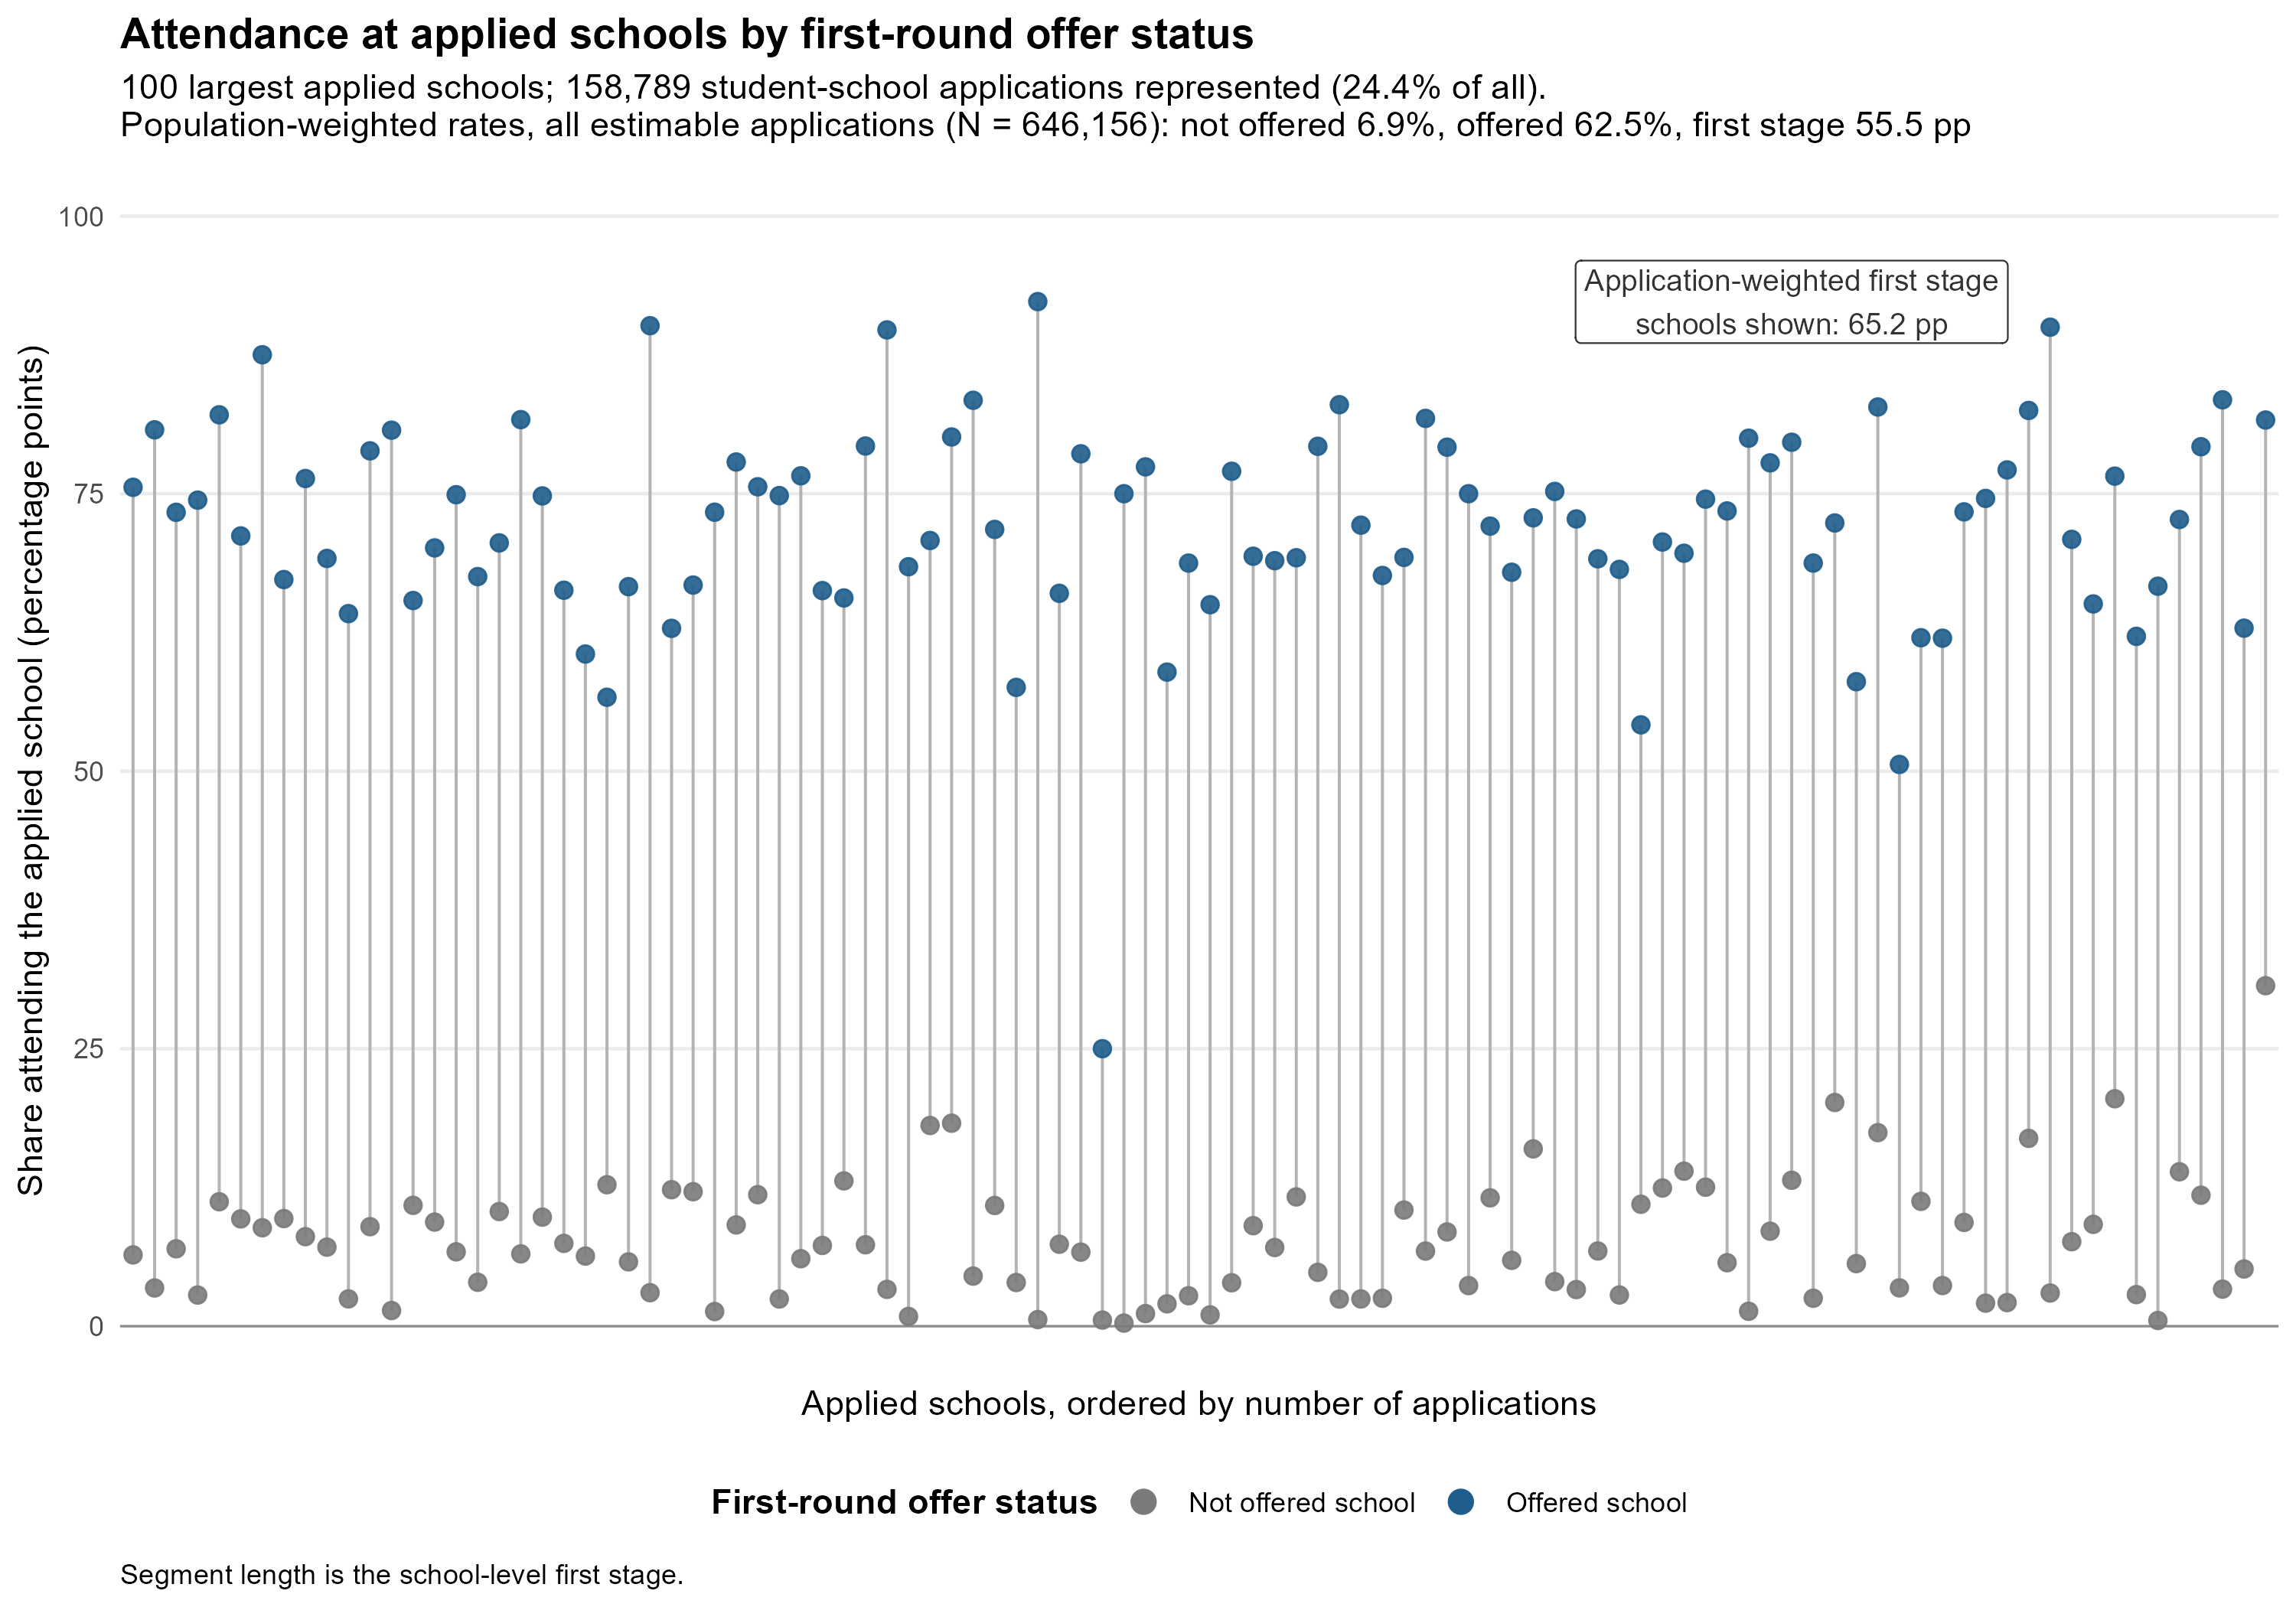
\includegraphics[width=\textwidth]{../../output/figures/compliance/school_level_offer_attendance_first_stage_top100.png}
\caption{Effect of SAE offers on attendance}
\label{fig:first-stage}
\begin{minipage}{\textwidth}
\footnotesize \textit{Notes:} The figure shows attendance rates at the 100 most demanded schools among timely SAE applicants with assignment risk, separately by whether the applicant received a first-round offer from that school. Attendance is the school in which the student spent the most time after grade 8; schools are ordered by applicant demand.
\end{minipage}
\end{figure}


For this exercise and the rest of the paper, I define high-school attendance as the school where a student spends the most time after grade 8, with most recent spells breaking ties.
This definition smooths over short enrollment spells and transfers, and it assigns a single high-school value to each student.
As a result, students who did not receive a first-round offer might still end up attending a certain high-school via complementary rounds or an application cycle in a later year.
On average, a high school is attended by 6.9\% of students rejected from it in the first round and by 62.5\% of students offered a seat.
The resulting difference of approximately 55.6 percentage points establishes a strong first stage for school attendance.



%The estimation sample consists of timely SAE applicants: students who apply in the assignment process corresponding to their grade-8 cohort and who have assignment risk in the simulated data.
%Assignment risk means that the simulated assignment probabilities do not place all probability mass on a single school.


%As shown in Table~\ref{tab:data-samples}, 135,916 students across the 2018--2020 cohorts have a valid high-school exposure, are ages 12--16, have complete lottery controls, apply to SAE on time, and face assignment risk.
%The score-based estimation sample further restricts to the 108,418 lottery-risk students with an observed math or verbal national admission-test score.
%On average, these students have positive simulated assignment probability at about 3.1 schools; the median is 3 and the 90th percentile is 5.

%Among applicants with assignment risk, 85.4\% receive a first-round SAE offer.
%The remaining 14.6\% have no first-round assignment (\texttt{rbd\_admitido}) in the regular-process results; they are retained, with their first-round offer value set to zero.
%The first-round offered RBD is the source of lottery variation, while the student's realized high-school exposure is measured by the most-time RBD described above.

%The value-added exercise uses the broader complete-control panel, while the causal estimates use the smaller lottery-risk sample.
%This distinction is central to the interpretation.
%The broad panel improves precision in estimating school-level outcome gradients, and the lottery sample then tests whether those observational value-added measures have causal signal on the centralized-assignment margin.
%The results therefore speak most directly to students and schools represented in the SAE lottery-risk sample.
%Because SAE covers the public and private-subsidized sector, this is a large and policy-relevant part of the high-school market, but extrapolating to private non-subsidized schools or non-lottery margins requires assuming that the same value-added gradients are comparable there.


\subsection{Sample Description}

This subsection describes the two samples used in the analysis.
The first is the value-added sample, a broad student panel used to estimate outcome-specific school fixed effects after adjusting for a rich set of covariates.
The second is the lottery sample, which contains students whose timely grade-9 SAE applications generate nondegenerate assignment probabilities.
I use this second sample to test whether lottery-induced changes in attended-school value added produce the outcome gains predicted by the observational measures.


\subsubsection{Value Added Sample}

I construct the value added sample by merging annual enrollment, grade progression, attendance, grades, and completion records using the student identifier provided for educational data.
The linked administrative panel starts from the universe of students observed in grade 8 between 2017 and 2020, producing 944,510 students across four cohorts defined by their year of grade-8 enrollment.
For instance, a student in the 2019 cohort who wants to change schools within the non-private system applies to SAE that year, is expected to start high school in 2020, and is expected to graduate in 2023.

%If a student in cohort 2019 intends to attend high school in a non private institution 
% is expected to apply that year to the centralized assignment mechanism for entrance to grade 9 in 2020 and has expected graduation in 2023.

To construct school value added, I retain as much of this broad panel as possible while imposing the restrictions required for comparable high-school exposure and baseline controls.
From this universe I drop students younger than 12 or older than 16 in grade 8 and those who do not attend high school. 


Requiring a complete vector of baseline covariates is the most consequential sample restriction.
For these covariates, I use information from Chile's national standardized assessment system (SIMCE) and middle school relative performance.
Middle school controls are constructed by comparing attendance and GPA of a student to those of their peers in middle school every year. 
These are then averaged and summarized into two middle school z-scores for a student: one for attendance and one for GPA.

SIMCE exams are administered in different grades depending on the year. 
This always includes grade 4 and occasionally grades 8 and/or 10.
Unfortunately grade-8 and grade-10 measures are not available for all the studied cohorts.
I therefore use grade-4 SIMCE as the main pre-treatment achievement control.

SIMCE also collects parent surveys.
I use these surveys to measure family background before treatment, including household income, parental education, indigenous origin of the parents, and early-childhood education.
These variables are useful because they proxy for family resources and prior investments that may influence both high-school choices and later higher-education outcomes.
When parent-survey variables are missing, I use middle school and neighborhood cells to impute medians where enough donor observations are available; remaining missing values are left missing.


%I define a middle school --with a similar role  for those students that can be tracked in the anual enrollment database, 
As shown in Panel A of Table \ref{tab:data-samples}, I retain 757,999 of the original 944,510 students with a valid high-school exposure, the required age range, and the complete control vector described above.
Sample restrictions defined in each row should be read cumulatively within each panel.



\begin{table}[H]
\centering
\caption{Construction of the value-added and SAE samples}
\label{tab:data-samples}
\begin{minipage}[t]{0.48\textwidth}
\centering
\textbf{Panel A: Value-added sample}\\[0.4em]
\begin{tabular}{@{}p{0.72\linewidth}r@{}}
\toprule
Sample restriction & Students \\
\midrule
Cohorts 2017--2020 & 944,510 \\
+ valid HS and age 12--16 & 931,547 \\
+ complete VA control set & \textbf{757,999} \\
+ admission test & 622,809 \\
\bottomrule
\end{tabular}
\end{minipage}
\hfill
\begin{minipage}[t]{0.48\textwidth}
\centering
\textbf{Panel B: SAE lottery sample}\\[0.4em]
\begin{tabular}{@{}p{0.72\linewidth}r@{}}
\toprule
Sample restriction & Students \\
\midrule
Cohorts 2018--2020 & 706,042 \\
+ valid HS and age 12--16 & 696,817 \\
+ complete lottery control set & 587,142 \\
+ application in SAE & 241,490 \\
+ assignment risk & \textbf{135,916} \\
+ admission test & 108,418 \\
\bottomrule
\end{tabular}
\end{minipage}
\end{table}



\subsubsection{Lottery Sample}


For the lottery sample, I follow the same initial steps using the 2018--2020 cohorts, the first cohorts for which SAE operated nationally.
Panel B of Table \ref{tab:data-samples} repeats the accounting exercise above for the lottery sample. 
Of the 706,042 students in these cohorts, 587,142 have a valid high-school exposure, fall within the required age range, and have the complete lottery control set.
Among them, 241,490 applied through SAE for a grade-9 seat while in grade 8.\footnote{I consider only applications to grade 9 in the year the student is in grade 8, to avoid including students who changed schools after repeating a grade.}
In some cases, students (e.g., those applying to undersubscribed schools) are guaranteed an offer to a certain school. 
The assignment mechanism does not yield exogenous variation for such cases since there is no tie-breaking.
The resulting lottery sample contains 135,916 students whose preferences and priorities imply nondegenerate assignment probabilities.



%For the value-added sample, I then retain the 2017--2020 cohorts, leaving 944,510 students across four cohorts.
%I make this cohort restriction because these cohorts have comparable grade-4 SIMCE baseline controls; the 2021 cohort does not.
%The main high-school exposure is observed for 4,133 schools with a unique identifier (RBD).
%I define high-school exposure as the school identifier where a student spends the most time after grade 8.
%I define middle-school attendance analogously as the RBD where the student spends the most time in grades 5 to 8.
%The same histories let me construct pre-treatment middle-school controls, including standardized measures of grades and attendance before high school.


%Table~\ref{tab:data-samples} summarizes how the linked administrative sources map into the two samples used in the analysis.
The broad complete-control panel is used to estimate the school value-added measures, while the 135,916 students with assignment risk form the base validation sample.
Math and verbal specifications additionally require an observed admission-test score, whereas the binary access and higher-education-choice outcomes retain non-test-takers whenever their outcome status can be defined.

\subsection{Characterization of the samples}

\textit{How different are these two samples?} Table \ref{tab:balance_samples} compares baseline characteristics and outcomes across the broad panel, all timely SAE applicants, and applicants with assignment risk.
Columns (1), (2), and (4) report group means; columns (3), (5), and (6) report the differences between SAE applicants and the broad panel, at-risk applicants and the broad panel, and at-risk applicants and all SAE applicants, respectively.

\begin{table}[H]
\centering
\caption{Balance across analysis samples}
\label{tab:balance_samples}
\scriptsize
\setlength{\tabcolsep}{2pt}
\begin{tabular}{@{}lcccccc@{}}
\toprule
 & \shortstack{Broad Panel\\(All HS)} & \multicolumn{2}{c}{SAE Applicants} & \multicolumn{2}{c}{SAE Applicants w/ risk} & \shortstack{Risk SAE -\\All SAE} \\
\cmidrule(lr){3-4} \cmidrule(lr){5-6}
 & Mean & Mean & \shortstack{Diff.\\(2)-(1)\\(SE)} & Mean & \shortstack{Diff.\\(4)-(1)\\(SE)} & \shortstack{Diff.\\(4)-(2)\\(SE)} \\
 & (1) & (2) & (3) & (4) & (5) & (6) \\
\midrule
\multicolumn{7}{l}{\textit{Student characteristics}} \\[2pt]
Female & 0.492 & 0.484 & -0.008 (0.001) & 0.495 & 0.004 (0.001) & 0.011 (0.001) \\
Metropolitan Region (Santiago) & 0.387 & 0.257 & -0.130 (0.001) & 0.273 & -0.114 (0.001) & 0.016 (0.001) \\
Age & 13.4 & 13.4 & 0.000 (0.001) & 13.3 & -0.035 (0.001) & -0.035 (0.001) \\
\midrule
\multicolumn{7}{l}{\textit{Baseline SIMCE variables}} \\[2pt]
Math 4th grade (z) & 0.036 & -0.232 & -0.268 (0.002) & -0.159 & -0.195 (0.002) & 0.073 (0.002) \\
Verbal 4th grade (z) & 0.036 & -0.189 & -0.225 (0.002) & -0.115 & -0.151 (0.002) & 0.074 (0.002) \\
Income decile & 5.5 & 4.5 & -0.991 (0.005) & 4.8 & -0.721 (0.006) & 0.271 (0.004) \\
Mother education years & 11.9 & 10.9 & -1.002 (0.005) & 11.2 & -0.709 (0.007) & 0.292 (0.005) \\
\quad\footnotesize{\% matched all SIMCE vars} & \footnotesize{82.4\%} & \footnotesize{81.8\%} &  & \footnotesize{83.4\%} &  &  \\
\midrule
\multicolumn{7}{l}{\textit{Middle school}} \\[2pt]
GPA (z) & 0.032 & 0.024 & -0.008 (0.001) & 0.093 & 0.061 (0.002) & 0.069 (0.001) \\
Attendance (z) & 0.021 & 0.030 & 0.009 (0.001) & 0.043 & 0.022 (0.002) & 0.014 (0.001) \\
\quad\footnotesize{\% matched all middle-school vars} & \footnotesize{99.8\%} & \footnotesize{99.8\%} &  & \footnotesize{99.8\%} &  &  \\
\midrule
\multicolumn{7}{l}{\textit{Outcomes}} \\[2pt]
Std. math exam & 0.000 & -0.334 & -0.334 (0.002) & -0.289 & -0.289 (0.002) & 0.045 (0.001) \\
Std. verbal exam & 0.000 & -0.301 & -0.301 (0.002) & -0.230 & -0.230 (0.003) & 0.072 (0.002) \\
Admission exam taker & 0.776 & 0.738 & -0.038 (0.001) & 0.769 & -0.007 (0.001) & 0.031 (0.001) \\
Higher ed. enrolled & 0.672 & 0.580 & -0.092 (0.001) & 0.617 & -0.055 (0.001) & 0.037 (0.001) \\
Hi-premium institution & 0.128 & 0.056 & -0.072 (0.000) & 0.067 & -0.061 (0.001) & 0.011 (0.000) \\
Hi-premium field & 0.307 & 0.258 & -0.048 (0.001) & 0.280 & -0.026 (0.001) & 0.022 (0.001) \\
\midrule
$N$ & 931,547 & 294,198 & & 162,633 & & \\
Percent of broad panel & 100.0\% & 31.6\% & & 17.5\% & & \\
Joint test $p$-value & & & $<0.001$ & & $<0.001$ & $<0.001$ \\
\bottomrule
\end{tabular}
\par\medskip\footnotesize
\begin{minipage}{\textwidth}
\textit{Notes:} The Broad Panel contains 2017--2020 cohorts with an observed high school and age 12--16. SAE Applicants are timely 2018--2020 grade-9 applicants; \textit{w/ risk} requires $\max_j p_{ij}<1$. Difference columns report the indicated mean differences, with overlap-adjusted standard errors in parentheses. Joint tests cover the baseline characteristics above the Outcomes section.
\end{minipage}
\end{table}



Column (3) shows that SAE applicants are negatively selected relative to the broad panel.
Their grade-4 math and verbal scores are 0.27 and 0.23 standard deviations lower, their household income is about one decile lower, and their mothers have approximately one fewer year of education.
Column (5) shows the same broad pattern for applicants with assignment risk, although the differences are smaller.
Column (6) confirms that at-risk applicants are positively selected relative to the full set of SAE applicants on these baseline measures.
The joint tests reject equality of the baseline characteristics in all three comparisons.

These differences matter because the observational value-added measures are estimated in the broad panel but validated among SAE applicants with assignment risk.
The validation exercise therefore asks directly whether school rankings estimated in the population represented by column (1) predict causal effects for the population represented by column (4), after controlling for the observed baseline characteristics used in the lottery specification.


\subsection{Higher Education Outcomes}

The seven primary outcomes are organized into the same three groups used throughout the results tables: \textit{achievement}, \textit{postsecondary access}, and \textit{within higher-education choice}.

The achievement group contains math and verbal scores from the national higher-education admission exam.
Taking this exam is itself a choice, but it is the standard route into selective higher education.
Applicants take mandatory math and verbal components and may also take optional subject exams.\footnote{The national admission exam was called the PSU through 2020, the PTU in 2021--2022, and the PAES from 2023 onward.}
I standardize math and verbal scores within test year to make them comparable across test regimes; these two outcomes are consequently observed only for exam takers.

The postsecondary-access group contains three binary outcomes defined for the broader eligible student population.
The first is admission-exam taking.
The second is whether the student submitted any application through the centralized state system for higher-education scholarships and student credit (FUAS).
The third is whether the student appears in the higher-education enrollment records.
Students who do not take the exam, submit a financial-aid application, or enroll are coded zero for the respective outcome.

The final group describes within-higher-education choices: whether a student enrolls in a high-premium institution and whether a student enrolls in a high-premium field.
Higher-education applications and admissions are organized at the program--institution level, so the enrollment records identify both the institution and field associated with a student's first observed enrollment.

Students in the sample have not yet finished higher education, so I cannot observe their realized earnings.
I instead use MiFuturo, an information source maintained by the Ministry of Education that reports program-level labor-market statistics, including average income in the fourth year after graduation.
Because MiFuturo identifiers do not map one-to-one into every program code in the enrollment records, I estimate a log-income model with institution and generic-program fixed effects.
These estimates provide a common measure of the earnings premium associated with each institution and generic program.
Figure~\ref{fig:mifuturo-field-income-premia} shows the generic-program fixed effects organized by field.

\begin{figure}[!htbp]
\centering
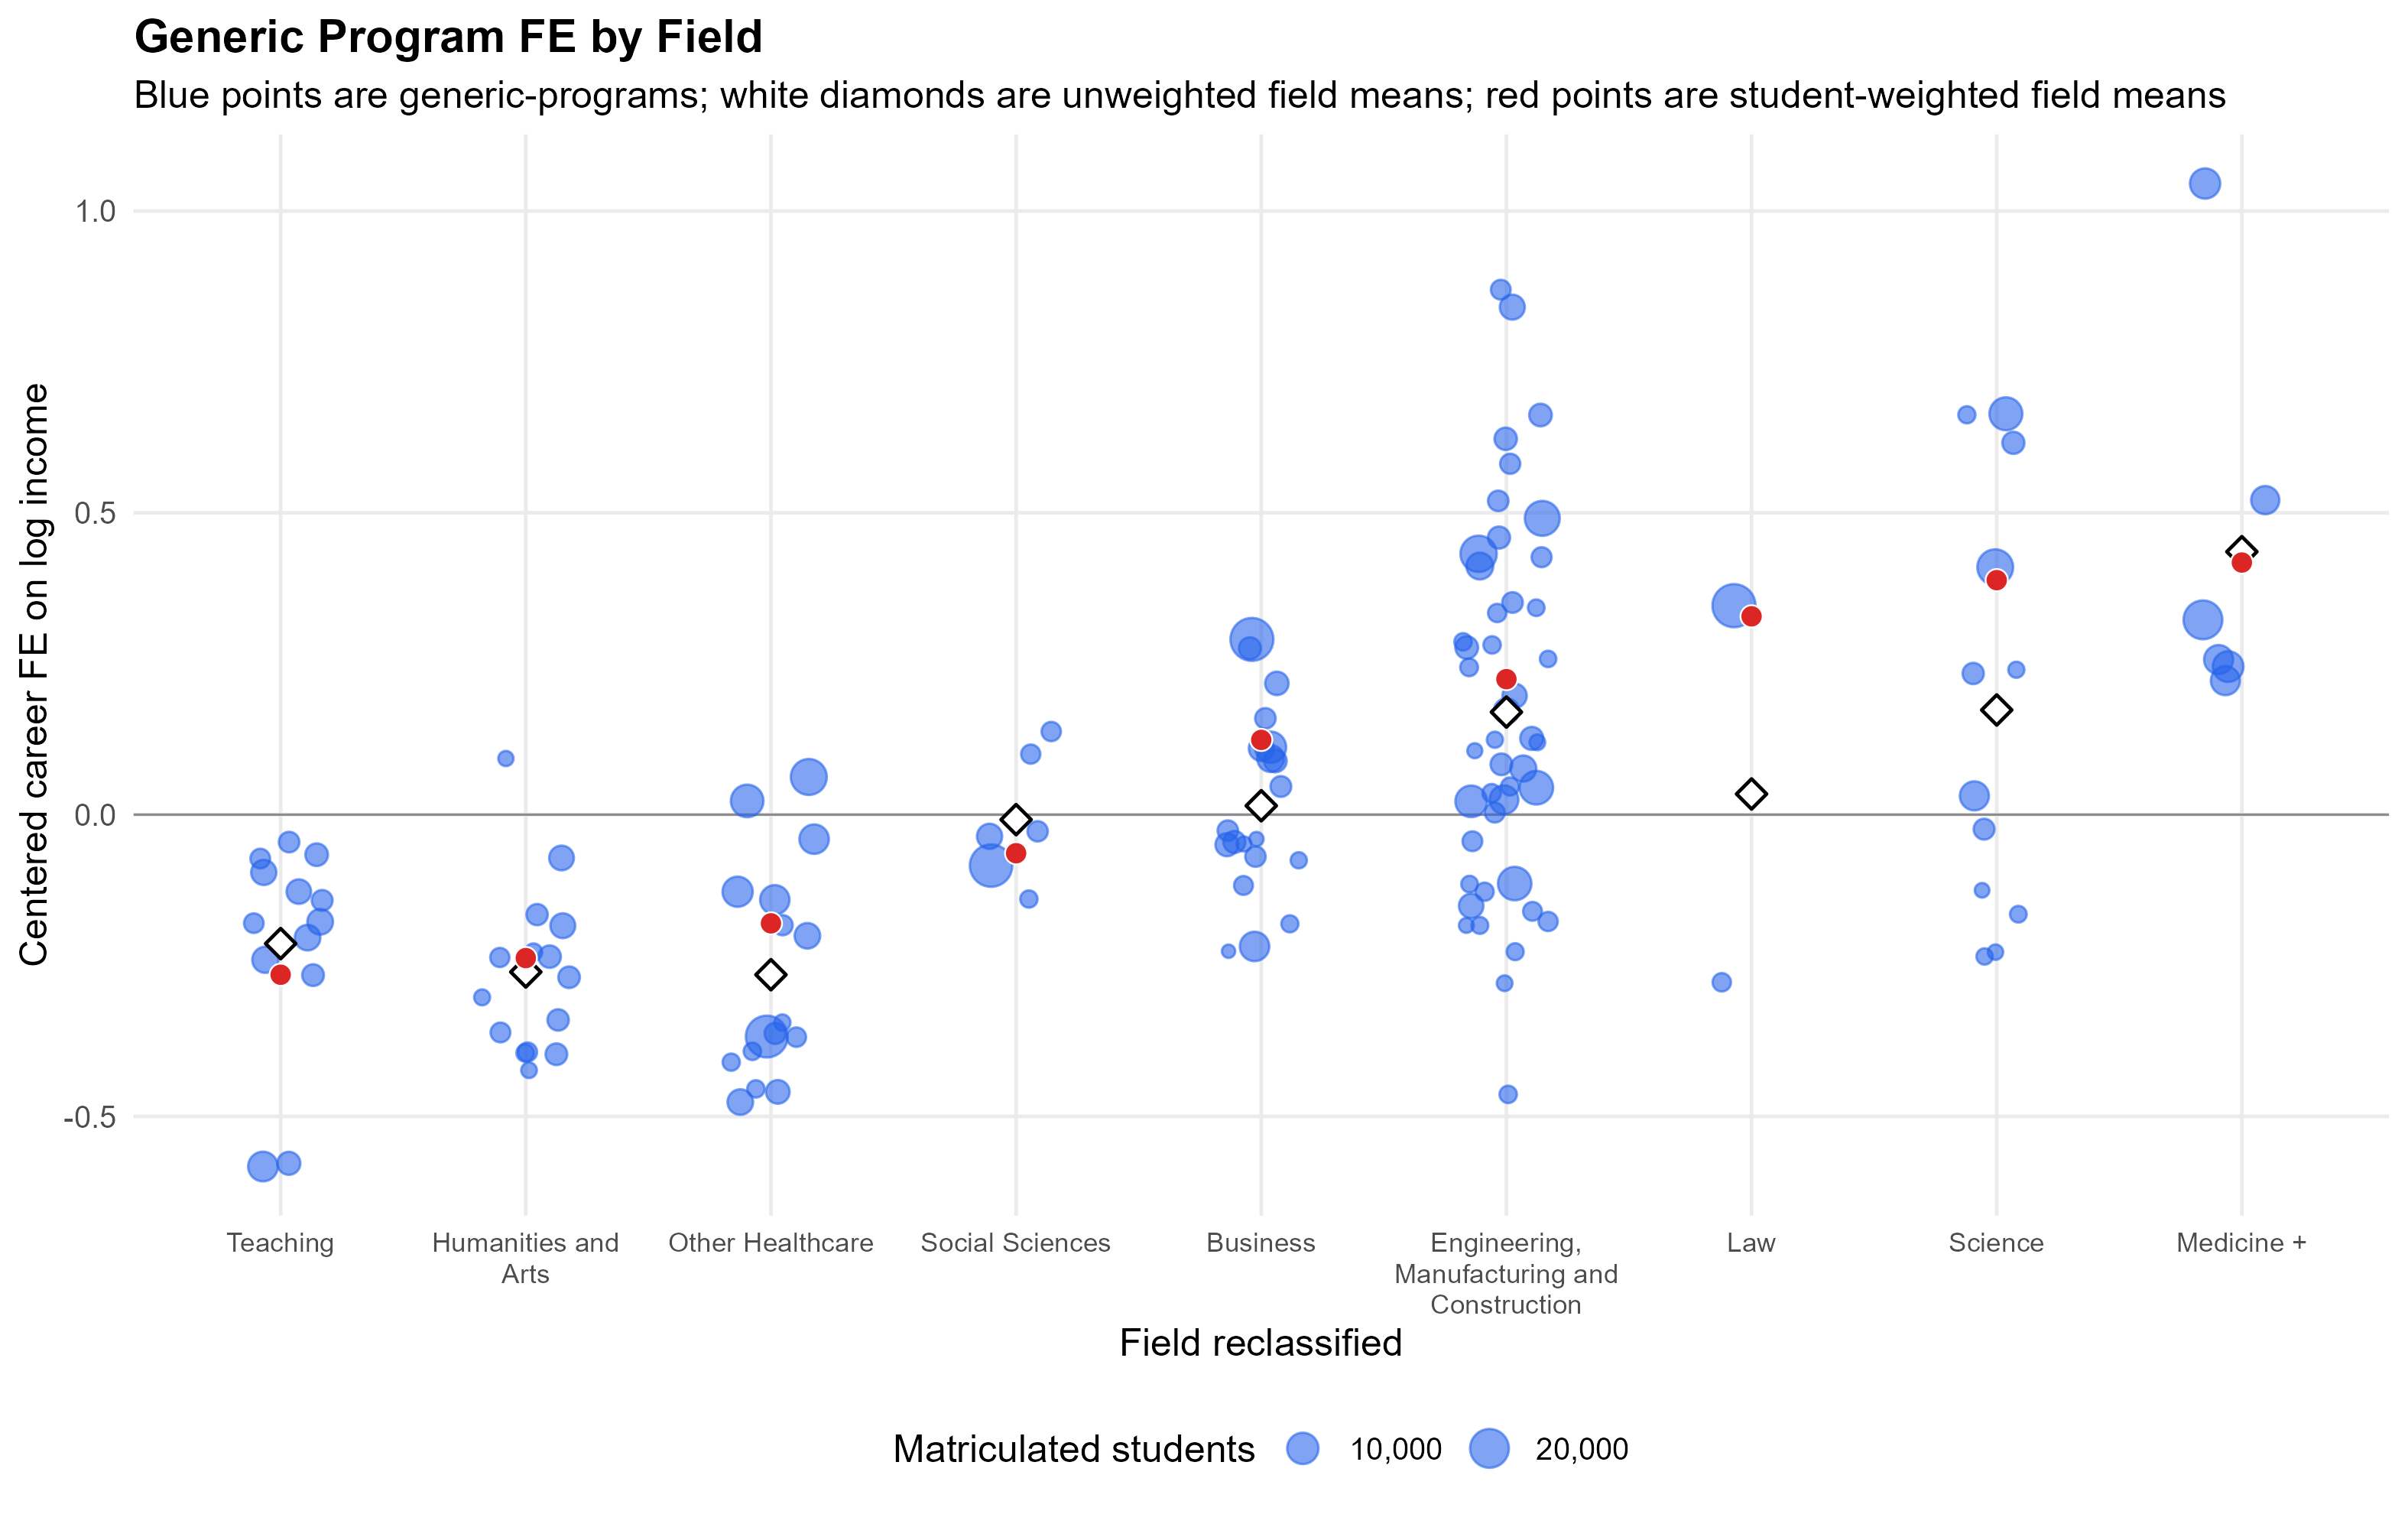
\includegraphics[width=\textwidth]{../../output/figures/mifuturo_matricula_income/area_carrera_generica_program_fe_by_field.png}
\caption{MiFuturo Generic-Program Income Premia by Field}
\label{fig:mifuturo-field-income-premia}
\begin{minipage}{\textwidth}
\footnotesize \textit{Notes:} The figure plots generic-program fixed effects from a log-income model with institution and generic-program effects, using MiFuturo earnings measured in the fourth year after graduation. Points are grouped by the field classification used in the analysis; higher values indicate programs associated with higher projected earnings, conditional on institution.
\end{minipage}
\end{figure}

The high-premium-field indicator equals one when the student's first observed enrollment is in Science, Law, Engineering/Manufacturing/Construction, or Medicine+.\footnote{Medicine+ includes medicine, pharmacy, nursing, midwifery, medical technology, and dentistry. Other health and technical-health programs are not included in the high-premium-field category.}
All other observed fields, including programs outside the retained field taxonomy, are coded zero.
The high-premium-institution indicator equals one when the institution associated with the student's first observed enrollment has a centered MiFuturo institution fixed effect above 0.1 log points.\footnote{A difference of 0.1 log points corresponds approximately to a 10\% institution premium. Matriculated students whose institution lacks an estimable fixed effect are coded zero.}

The phrase ``within higher-education choice'' describes the information used to construct these two outcomes: an institution or field can be classified only when an enrollment choice is observed.
The outcomes used in the main regressions are nevertheless unconditional with respect to higher-education enrollment.
Students without an observed higher-education enrollment are coded zero rather than removed from the sample.
Both the observational value-added construction and the lottery IV specifications for these two outcomes are restricted to admission-exam takers.
The resulting coefficients therefore combine an effect on the probability of entering higher education with an effect on the type of institution or field chosen upon enrollment; they should not be interpreted as effects conditional on enrollment.
Estimating the latter object would require conditioning on a post-assignment outcome that schools may themselves affect.


\clearpage

\section{Empirical Framework}
\label{sec:framework}

This section describes the empirical objects and research design. The goal is not to
estimate a separate causal effect for every school and every possible margin of
substitution. Instead, I ask whether outcome-specific observational measures of school
value added predict causal effects generated by lottery-induced changes in high-school
attendance. The design therefore summarizes school effectiveness with scalar
outcome-specific indices and estimates a forecast coefficient for each outcome.


\subsection{School Effects and Observational Value Added}

I use a constant-effects value-added model as a guide. Let

\begin{equation}
    Y_i^m(j)
    =
    \mu^m + V_j^m + \epsilon_i^m,
    \label{eq:potential-va}
\end{equation}

where $Y_i^m(j)$ is student $i$'s potential outcome for outcome $m$ if student $i$
attends high school $j$. The term $\mu^m$ denotes the average level of outcome $m$,
and $V_j^m$ is the causal contribution of school $j$ to that outcome relative to the
student-weighted average school. I normalize
\[
    \sum_j \omega_j V_j^m = 0,
\]
where $\omega_j$ is the share of students attending school $j$ in the value-added
sample. A positive $V_j^m$ therefore denotes a school with an above-average causal
effect on outcome $m$.

The main outcomes considered in the paper are math and verbal achievement;
admission-exam taking, financial-aid application, and higher-education enrollment;
and enrollment in a high-premium institution or field.

The causal effects $V_j^m$ are not directly observed. I first construct observational
measures of school value added using the broad complete-control panel. For each
outcome $m$, consider the population regression

\begin{equation}
    Y_i^m
    =
    \alpha^m
    +
    \lambda_{s(i)}^m
    +
    X_i'\Gamma^m
    +
    u_i^m,
    \label{eq:observational-va}
\end{equation}

where $s(i)$ denotes the high school attended by student $i$, and $X_i$ contains
pre-treatment characteristics. These include cohort, gender, age, a third-degree
polynomial in grade-4 SIMCE math and language scores, family-background measures
from SIMCE parent surveys,\footnote{In particular, family income decile, years of
education and indigenous status of each parent, and indicators for whether the student
attended an educational institution before primary school.} and middle-school controls
constructed from grades 5 through 8, including school-normalized attendance and
academic performance.

I normalize the population observational school effects using the same student weights,
so that
\[
    \sum_j \omega_j \lambda_j^m = 0.
\]
I estimate equation~\eqref{eq:observational-va} and define
$\widehat V_j^m$ as the corresponding centered estimate of $\lambda_j^m$.

The distinction between $\lambda_j^m$ and $V_j^m$ is important. The former describes
conditional differences in outcomes across schools in the observational population,
whereas the latter denotes the causal effect of attending school $j$. If school attendance
were conditionally mean independent of potential outcomes given $X_i$, the two objects
would coincide. In practice, students and families sort across high schools, so
$\lambda_j^m$ may also reflect residual selection not absorbed by the controls.

The lottery validation below therefore asks whether differences in observational school
value added predict differences in causal school effects. In particular, I ask whether the
component of $\widehat V_j^m$ shifted by the centralized assignment mechanism produces
changes in outcome $m$ of the magnitude predicted by the observational measure.


\subsection{Assignment Risk and Offer Shocks}

SAE applicants submit rank-ordered lists of schools. Let $\mathcal J$ denote the set of high
schools and let $\mathcal J_0=\mathcal J\cup\{0\}$, where $0$ denotes no first-round offer.
Let $Z_i\in\mathcal J_0$ denote student $i$'s first-round offer and set
$\widehat V_0^m=0$. Let $D_i\in\mathcal J$ denote the high school ultimately attended,
measured by the post-grade-8 most-time RBD.

For each possible offer $z$, let $D_i(z)$ denote the school that student $i$ would attend
if offered school $z$. Let $Y_i^m(d)$ denote the potential outcome under attendance at
school $d$, and let $Y_i^m(z)$ denote the potential outcome under offer $z$. The assignment
mechanism maps each student's submitted preferences and priorities, denoted by $\theta_i$,
into the full offer-probability vector
\[
    p_i=(p_{ij})_{j\in\mathcal J_0},
    \qquad
    p_{ij}=\Pr(Z_i=j\mid\theta_i),
\]
where the probability is taken over repeated draws of the randomized tie-breakers, holding
$\theta_i$ fixed. This use of the assignment mechanism to isolate lottery variation follows
\textcite{abdulkadiroglu_research_2017}; its application to school value-added validation
follows \textcite{angrist_methods_2023}. Let $W_i$ denote the predetermined controls used below.

\begin{assumption}[Offer exogeneity and exclusion]
\label{ass:lottery}

\textit{Offer exogeneity.} For each outcome $m$, conditional on $p_i$, the realized first-round offer is independent
of predetermined controls and the joint schedules of potential attendance choices and
potential outcomes:
\[
    Z_i
    \perp\!\!\!\perp
    \left(
        \{D_i(z)\}_{z\in\mathcal J_0},
        \{Y_i^m(d)\}_{d\in\mathcal J},
        W_i
    \right)
    \mid p_i .
\]

\textit{Exclusion.} Offers have no direct effect on outcomes beyond the school attended:
\[
    Y_i^m(z)=Y_i^m\!\left(D_i(z)\right)
    \qquad
    \text{for every }z\in\mathcal J_0.
\]
\end{assumption}

Offer exogeneity is the conditional-independence restriction. Rankings and priorities are
fixed before SAE draws the random tie-breakers, and $p_i$ records the resulting distribution
of possible offers. The restriction therefore allows preferences, priorities, and $p_i$ to
be arbitrarily related to potential outcomes; it requires the realized draw to be random
within that assignment risk. Exclusion separately requires that an offer affect outcome $m$
only by changing the high school attended.

The complete vector $p_i$ is high-dimensional because students submit different rankings
and face different priorities and capacities. For an outcome-specific scalar value-added
measure, I summarize this assignment risk using the expected value added of the offered
school:

\begin{equation}
    E_i^m
    =
    \sum_{j\in\mathcal J_0}p_{ij}\widehat V_j^m.
    \label{eq:expected-va}
\end{equation}

This is the average observational value added of the offer student $i$ would receive over
repeated randomizations of the assignment mechanism, holding the student's application
and priorities fixed.

Define the observational value added of the school attended and the school offered as

\begin{equation}
    A_i^m
    =
    \widehat V_{D_i}^m,
    \qquad
    O_i^m
    =
    \widehat V_{Z_i}^m.
    \label{eq:attended-offered-va}
\end{equation}

Because
\[
    O_i^m=\widehat V_{Z_i}^m,
\]
its conditional expectation under the assignment mechanism is

\begin{equation}
    \mathbb E[O_i^m\mid p_i]
    =
    \sum_{j\in\mathcal J_0}p_{ij}\widehat V_j^m
    =
    E_i^m.
    \label{eq:offer-expectation}
\end{equation}

Following the recentering logic of \textcite{borusyak_nonrandom_2023}, define the
outcome-specific offer shock
\begin{equation}
    \widetilde O_i^m
    \equiv
    O_i^m-E_i^m.
    \label{eq:offer-shock}
\end{equation}
Let $\mathcal S_i^m$ collect the potential attendance schedule, potential outcome schedule,
and $W_i$. Holding the estimated school index and simulated assignment probabilities fixed,
offer exogeneity implies
\begin{align}
    \mathbb E[O_i^m\mid p_i,\mathcal S_i^m]
    &=
    \sum_{j\in\mathcal J_0}\widehat V_j^m
    \Pr(Z_i=j\mid p_i,\mathcal S_i^m) \notag\\
    &=
    \sum_{j\in\mathcal J_0}p_{ij}\widehat V_j^m
    =E_i^m,
    \label{eq:offer-exogeneity-moment}
\end{align}
and hence
\[
    \mathbb E[\widetilde O_i^m\mid p_i,\mathcal S_i^m]=0.
\]
The weaker equality $\mathbb E[\widetilde O_i^m\mid p_i]=0$ would establish only that the
offer shock is centered. The moment above establishes the required orthogonality to the
counterfactual attendance and outcome schedules, even when assignment risk is related to
them. The scalar $E_i^m$ is not assumed to replace the full $p_i$ as a balancing score.
It forms the conditional-mean residual of the scalar offer value; because the moment holds
at every $p_i$, it also holds after integrating over assignment risk. Exclusion ensures that
any reduced-form effect of this shock operates through the school attended.


\subsection{Scalar IV Specification}

The first empirical question is whether observational school value added forecasts causal
effects on the corresponding outcome. Specifically, when the assignment mechanism
induces a student to attend a school with higher $\widehat V_j^m$, does outcome $m$
improve, and by how much relative to the observational difference encoded in
$\widehat V_j^m$?

I estimate the following IV system:

\begin{equation}
    Y_i^m
    =
    \alpha^m
    +
    \psi^m A_i^m
    +
    \rho^m E_i^m
    +
    W_i'\delta^m
    +
    \eta_i^m,
    \label{eq:pass-through}
\end{equation}

with first stage

\begin{equation}
    A_i^m
    =
    a^m
    +
    \kappa^m \widetilde O_i^m
    +
    \rho_A^m E_i^m
    +
    W_i'\delta_A^m
    +
    \nu_i^m.
    \label{eq:first-stage}
\end{equation}

Here, $Y_i^m$ is student $i$'s realized outcome, $A_i^m$ is the observational value
added of the school attended, and $\widetilde O_i^m$ is the lottery-induced component of
the offered school's observational value added. The offer shock instruments for attended
value added, while $E_i^m$ controls for the level predicted by the student's assignment
probabilities. Because $O_i^m=\widetilde O_i^m+E_i^m$ and $E_i^m$ is included as a control,
this is algebraically identical to using $O_i^m$ as the excluded instrument.

The vector $W_i$ contains a parsimonious set of predetermined characteristics: cohort,
gender, age, and grade-4 SIMCE math and language scores. This differs from the richer
control vector used to construct $\widehat V_j^m$ in
equation~\eqref{eq:observational-va}, which additionally includes family-background and
middle-school characteristics. All reported specifications use heteroskedasticity-robust
standard errors.

Identification additionally requires a nonzero first stage:

\begin{equation}
    \operatorname{Cov}
    \left(
        \widetilde O_i^m,\,
        A_i^m
    \right)
    \neq 0.
    \label{eq:rank-condition}
\end{equation}

This relevance condition is assessed using the first-stage coefficients and excluded-instrument
$F$ statistics reported in Table~\ref{tab:scalar-school-value-iv-main-seven-eb-first-stage}.

The coefficient $\psi^m$ is the central parameter of the validation exercise. I refer to it
as the forecast coefficient, or interchangeably as pass-through. It measures the change in
outcome $m$ generated by a lottery-induced one-unit increase in the observational value
added of the school attended.

If $\psi^m=1$, the causal gain generated by lottery-induced movement across schools
matches the difference predicted by observational value added. If $\psi^m=0$, the
observational measure has no causal predictive content along the lottery-induced margin.
Values between zero and one indicate that observational value added is directionally
informative but that observational differences overstate the corresponding causal gains.

Importantly, $\psi^m$ should be interpreted as a causal forecast coefficient rather than
as the structural effect of a manipulable treatment called ``value added.'' The underlying
treatment is attendance at a different high school. The scalar index asks whether the
observational ranking of those schools predicts the causal consequences of the school
changes induced by the lottery.

The scalar specification is useful because a fully flexible school-specific IV design would
be high-dimensional and would combine many margins of substitution across fallback
schools \parencite{angrist_methods_2023,kirkeboen_field_2016}. The scalar design instead
asks whether movement toward schools with higher measured value added produces better
outcomes, after accounting for the assignment risk implied by each student's submitted
preferences and priorities.


\subsection{Empirical Bayes}

The observational school fixed effects in equation~\eqref{eq:observational-va} are
estimated with different degrees of precision. Estimates for schools with fewer students
or noisier outcomes contain more sampling error. Using the raw estimates therefore gives
rise to extreme values that may partly reflect estimation noise.

I use an Empirical-Bayes shrinkage procedure to improve the signal-to-noise ratio of the
school indices before using them in the lottery design
\parencite{walters_chapter_2024}. For each school $j$ and outcome $m$, let $se_j^m$
denote the regression-derived standard error of the centered fixed-effect estimate
$\widehat V_j^m$.

The EB calculation relies on the following sampling-error approximation.

\begin{assumption}[Sampling error in observational value added]
\label{ass:va_sampling}

For each school $j$ and outcome $m$,
\[
    \widehat V_j^m
    =
    \lambda_j^m + e_j^m,
\]
where $\lambda_j^m$ is the centered population observational school effect from
equation~\eqref{eq:observational-va}, and
\[
    \mathbb E
    \left[
        e_j^m
        \mid
        \lambda_j^m,se_j^m
    \right]
    =0,
    \qquad
    \operatorname{Var}
    \left(
        e_j^m
        \mid
        \lambda_j^m,se_j^m
    \right)
    =
    (se_j^m)^2.
\]
\end{assumption}

Assumption~\ref{ass:va_sampling} concerns sampling error in the estimated observational
school effects. It does not require the population observational effect $\lambda_j^m$ to
equal the causal school effect $V_j^m$. Whether observational school effectiveness
predicts causal school effectiveness is precisely the object of the lottery validation
exercise.

Under Assumption~\ref{ass:va_sampling}, the cross-school dispersion of the estimated
effects combines dispersion in population observational value added with estimation
noise. I therefore estimate the latent across-school variance as

\begin{equation}
    \widehat{\tau}_m^2
    =
    \max
    \left\{
        \operatorname{Var}_{\omega}
        \left(
            \widehat V_j^m
        \right)
        -
        \sum_j
        \omega_j
        (se_j^m)^2,
        \,
        0
    \right\},
    \label{eq:eb-latent-variance}
\end{equation}

where $\omega_j$ is proportional to the number of students in school $j$'s value-added
regression sample. I perform this calculation separately for each outcome using its
outcome-specific estimation sample and student weights.

To translate the estimated signal variance into school-specific shrinkage, I use a
normal--normal working model: population observational school effects are approximated
by a normal distribution with mean $\overline{\widehat V}_{\omega}^m$ and variance
$\widehat\tau_m^2$, and estimation error is approximated as normal with variance
$(se_j^m)^2$. This additional distributional approximation, together with
Assumption~\ref{ass:va_sampling}, yields the school-specific reliability weight

\begin{equation}
    r_j^m
    =
    \frac{\widehat{\tau}_m^2}
    {\widehat{\tau}_m^2+(se_j^m)^2}.
    \label{eq:eb-reliability}
\end{equation}

I first construct the posterior-mean school index

\begin{equation}
    \widetilde V_j^{m,EB}
    =
    \overline{\widehat V}_{\omega}^m
    +
    r_j^m
    \left(
        \widehat V_j^m
        -
        \overline{\widehat V}_{\omega}^m
    \right),
\end{equation}

where $\overline{\widehat V}_{\omega}^m$ is the student-weighted mean of the estimated
school effects. The raw estimates are centered, so this shrinkage target is zero up to
numerical precision. Because reliability varies across schools, however, the weighted
mean of the posterior means need not remain exactly zero. The implementation therefore
re-centers the posterior means using the same student weights:

\begin{equation}
    \widehat V_j^{m,EB}
    =
    \widetilde V_j^{m,EB}
    -
    \sum_k \omega_k\widetilde V_k^{m,EB}.
    \label{eq:eb-va}
\end{equation}

This final student-centered index is the EB measure reported in the distribution table
and used in the main lottery specifications.

As $se_j^m$ becomes small relative to $\widehat\tau_m$, reliability approaches one and
the preliminary posterior mean $\widetilde V_j^{m,EB}$ approaches the original estimate
$\widehat V_j^m$. Less precise school estimates are instead shrunk more strongly toward
the across-school mean. Under the normal--normal working model above,
$\widetilde V_j^{m,EB}$ is the Empirical-Bayes posterior mean;
$\widehat V_j^{m,EB}$ is its student-centered version.

For the main same-outcome scalar IV specifications, I replace the raw observational
school index with its EB-shrunken counterpart:

\begin{align}
    A_i^{m,EB}
    &=
    \widehat V_{D_i}^{m,EB},
    &
    O_i^{m,EB}
    &=
    \widehat V_{Z_i}^{m,EB},
    \notag\\
    E_i^{m,EB}
    &=
    \sum_{j\in\mathcal J_0}p_{ij}\widehat V_j^{m,EB},
    &
    \widetilde O_i^{m,EB}
    &=
    O_i^{m,EB}-E_i^{m,EB},
    \label{eq:eb-iv-objects}
\end{align}

Here the no-offer value is again zero. The EB specification instruments $A_i^{m,EB}$
with $\widetilde O_i^{m,EB}$ and controls for $E_i^{m,EB}$ exactly as in
equations~\eqref{eq:pass-through} and \eqref{eq:first-stage}.
The shrinkage step therefore changes the precision and scale of the observational school-quality index used by the lottery design; it does not itself identify causal school effects.
Accordingly, the null $\psi^{m,EB}=1$ tests whether the EB-shrunken index is calibrated to the lottery-induced outcome gain on its own scale.
The later comparison of direct IV estimates with RSS-implied cross-outcome gains instead uses unshrunk value added so that both objects are expressed on the same underlying value-added scale.


\subsection{Cross-Outcome Relationships in School Value Added}

To study whether school effectiveness is multidimensional, I estimate how latent
observational effects $\lambda_j^m$ and $\lambda_j^{m'}$ covary across outcomes
\parencite{jackson_what_2018, rose_effects_2022}. A covariance computed directly from
$\widehat V_j^m$ and $\widehat V_j^{m'}$ is biased when their sampling errors are correlated,
as can occur because the estimates use overlapping students. Outcome-by-outcome EB
shrinkage does not remove this cross-outcome noise.

I therefore adapt the cross-cohort estimator of \textcite{rose_effects_2022}. It uses
different cohorts to estimate the product $\lambda_j^m\lambda_j^{m'}$, avoiding covariance
between sampling errors measured in the same cohort.

Formally, let $t \in \{1,\ldots,T_j\}$ index the grade-8 cohorts observed for school $j$ (cohorts 2017--2020), and define the school-by-cohort mean of the fitted residual plus school effect from equation~\eqref{eq:observational-va}:
\begin{equation}
  \widehat\lambda_{jt}^m = \frac{1}{n_{jt}^m}\sum_{i:\, s(i)=j,\, c(i)=t} \left(\widehat\lambda_j^m + \widehat u_i^m\right) = \lambda_j^m + \bar e_{jt}^m,
  \label{eq:varcov-cell-mean}
\end{equation}
where $c(i)$ is the grade-8 cohort and $E[\bar e_{jt}^m]=0$. These components use the
same controls and fixed effects as equation~\eqref{eq:observational-va}.

\begin{assumption}[Uncorrelated cross-cohort sampling error]
  For any school $j$ and any two cohorts $t\neq t'$, and for any pair of outcomes $m, m'$ (including $m=m'$),
  $E\left[\bar e_{jt}^m \bar e_{jt'}^{m'}\right]=0$.
  \label{as:cross-cohort}
\end{assumption}

The assumption permits correlated errors across outcomes within a cohort but rules out
correlated errors across cohorts of the same school. Cross-cohort products then identify
products of latent school effects. For an own-outcome variance, define
\begin{equation}
  S_j^{m,m}
  =
  \frac{\left(\sum_t\widehat\lambda_{jt}^m\right)^2-
  \sum_t\left(\widehat\lambda_{jt}^m\right)^2}
  {T_j^m(T_j^m-1)},
  \qquad
  \overline{\widehat\lambda}_j^m
  =
  \frac{1}{T_j^m}\sum_t\widehat\lambda_{jt}^m.
  \label{eq:varcov-school-signal}
\end{equation}
For two outcomes, let $\mathcal P_j^{m,m'}$ contain the ordered cohort pairs $(t,t')$ available
for school $j$ with $t\neq t'$, and define
\begin{equation}
  S_j^{m,m'}
  =
  \frac{1}{|\mathcal P_j^{m,m'}|}
  \sum_{(t,t')\in\mathcal P_j^{m,m'}}
  \widehat\lambda_{jt}^m\widehat\lambda_{jt'}^{m'}.
  \label{eq:varcov-school-cross-signal}
\end{equation}
Thus $E[S_j^{m,m'}]=\lambda_j^m\lambda_j^{m'}$, including when $m=m'$. I aggregate
these signals using student weights. Pairwise variances and covariances use the same schools
and weights; eligible schools must appear in at least two cohorts for each relevant outcome.
Suppressing outcome superscripts on the normalized weights, the estimators are
\begin{equation}
  \widehat{\mathrm{Var}}_{\omega}\left(\lambda^m\right)
  =
  \sum_j \omega_j(1-\omega_j)S_j^{m,m}
  -
  \sum_{j\neq k}\omega_j\omega_k
  \overline{\widehat\lambda}_j^m
  \overline{\widehat\lambda}_k^m,
  \label{eq:varcov-variance}
\end{equation}
\begin{equation}
  \widehat{\mathrm{Cov}}_{\omega}\left(\lambda^m,\lambda^{m'}\right)
  =
  \sum_j \omega_j(1-\omega_j)S_j^{m,m'}
  -
  \sum_{j\neq k}\omega_j\omega_k
  \overline{\widehat\lambda}_j^m
  \overline{\widehat\lambda}_k^{m'},
  \label{eq:varcov-covariance}
\end{equation}

Under Assumption~\ref{as:cross-cohort}, these expressions target the latent variance and
covariance directly. I summarize them with the cross-outcome correlation
\begin{equation}
  \widehat\rho^{\,m,m'} = \frac{\widehat{\mathrm{Cov}}_{\omega}\left(\lambda^m,\lambda^{m'}\right)}{\sqrt{\widehat{\mathrm{Var}}_{\omega}(\lambda^m)\,\widehat{\mathrm{Var}}_{\omega}(\lambda^{m'})}},
  \label{eq:varcov-correlation}
\end{equation}
and the directional projection of destination-outcome value added $m'$ on origin-outcome
value added $m$,
\begin{equation}
  \widehat\beta^{\,m' \mid m} = \frac{\widehat{\mathrm{Cov}}_{\omega}\left(\lambda^m,\lambda^{m'}\right)}{\widehat{\mathrm{Var}}_{\omega}(\lambda^m)}.
  \label{eq:varcov-implied-gain}
\end{equation}
$\widehat\beta^{\,m'\mid m}$ is the expected difference in latent value added on $m'$ associated
with a one-unit difference in latent value added on $m$. I estimate both objects for all
pairs among the seven primary outcomes, using the same outcome-specific samples as the
pooled VA exercise. They are descriptive until combined with the lottery pass-through
estimates in Section~4.4, where I assess whether they predict causal cross-outcome gains.

Inference uses a school-level nonparametric bootstrap. Each replicate jointly recomputes
the two variances and covariance entering a correlation or projection.

\clearpage

%\section{Characterizing applications and compliers}

% [FIX] Section 4 is a stub ('In this section', 'Table X sh'). Also the heading ('Characterizing applications and compliers') should be title-cased like the others.
%In this section 


%\subsection{Characterizing applications}

%\subsection{Characterizing compliers}


%\begin{table}[!htbp]
\centering
\caption{Baseline characteristics of math value-added compliers}
\label{tab:math-va-complier-ses}
\begin{threeparttable}
\small
\setlength{\tabcolsep}{4pt}
\begin{tabular}{lcccc}
\toprule
 & SAE mean & Above P25 & Above median & Above P75 \\
\midrule
Baseline math score & -0.233 & +0.025 & +0.151*** & +0.294*** \\
 &  & (0.020) & (0.016) & (0.024) \\
Baseline verbal score & -0.189 & +0.049** & +0.174*** & +0.325*** \\
 &  & (0.020) & (0.016) & (0.024) \\
Income decile & 4.519 & +0.142*** & +0.423*** & +0.615*** \\
 &  & (0.053) & (0.045) & (0.069) \\
Father's education (years) & 10.771 & +0.146** & +0.417*** & +0.764*** \\
 &  & (0.059) & (0.051) & (0.077) \\
Mother's education (years) & 10.941 & +0.163*** & +0.458*** & +0.768*** \\
 &  & (0.056) & (0.047) & (0.069) \\
\bottomrule
\end{tabular}
\begin{tablenotes}[flushleft]
\footnotesize
\item Notes: Each threshold column reports the estimated mean baseline characteristic among students induced by their first-round offer to attend a school above the stated math value-added threshold, minus the corresponding mean among all timely SAE applicants in the 2018--2020 cohorts. The SAE mean is common across thresholds. Parentheses contain heteroskedasticity-robust standard errors that account for estimation of the complier and population means and their covariance. High value added is defined using equally weighted school quantiles of EB-shrunken value added. The complier population and estimation sample may differ across thresholds. Differences describe baseline composition and are not treatment effects. $^{*}p<0.10$, $^{**}p<0.05$, $^{***}p<0.01$.
\end{tablenotes}
\end{threeparttable}
\end{table}



%\begin{table}[!htbp]
\centering
\caption{Baseline characteristics of high-premium-field value-added compliers}
\label{tab:high-premium-field-va-complier-ses}
\begin{threeparttable}
\small
\setlength{\tabcolsep}{4pt}
\begin{tabular}{lcccc}
\toprule
 & SAE mean & Above P25 & Above median & Above P75 \\
\midrule
Baseline math score & -0.233 & +0.053** & +0.088*** & +0.084*** \\
 &  & (0.024) & (0.017) & (0.015) \\
Baseline verbal score & -0.189 & +0.071*** & +0.083*** & +0.062*** \\
 &  & (0.024) & (0.017) & (0.015) \\
Income decile & 4.519 & +0.121* & +0.227*** & +0.314*** \\
 &  & (0.063) & (0.045) & (0.040) \\
Father's education (years) & 10.771 & +0.046 & +0.188*** & +0.321*** \\
 &  & (0.071) & (0.050) & (0.045) \\
Mother's education (years) & 10.941 & +0.152** & +0.251*** & +0.330*** \\
 &  & (0.067) & (0.048) & (0.043) \\
\bottomrule
\end{tabular}
\begin{tablenotes}[flushleft]
\footnotesize
\item Notes: Each threshold column reports the estimated mean baseline characteristic among students induced by their first-round offer to attend a school above the stated high-premium-field value-added threshold, minus the corresponding mean among all timely SAE applicants in the 2018--2020 cohorts. The SAE mean is common across thresholds. Parentheses contain heteroskedasticity-robust standard errors that account for estimation of the complier and population means and their covariance. High value added is defined using equally weighted school quantiles of EB-shrunken value added. The complier population and estimation sample may differ across thresholds. Differences describe baseline composition and are not treatment effects. $^{*}p<0.10$, $^{**}p<0.05$, $^{***}p<0.01$.
\end{tablenotes}
\end{threeparttable}
\end{table}



%Table X sh

%\clearpage 
\section{Causal Effects of Schools}
\label{sec:results}

 I organize the results in four blocks. 
 First, I describe the scale of the underlying outcomes and the distribution of the seven primary observational school value-added measures. 
 Second, I report the first-stage and pass-through estimates for each outcome. 
 Third, I relate the value-added measures to school organization and staff credentials. 
 Finally, I estimate the covariance structure of school value added and compare its implied cross-outcome gains with direct IV estimates.

\subsection{Distribution of Value-Added Estimates}

Table~\ref{tab:school-va-distribution} reports the scale of each student outcome and the dispersion of the corresponding school value-added measure for all seven primary outcomes. Binary outcomes and their value-added measures are expressed in percentage points, while achievement outcomes are expressed in standard deviations. For school value added, the table compares the posterior EB standard deviation and 90--10 gap with the dispersion of the unshrunk estimates and the cross-cohort RSS estimate of latent dispersion.

\begin{table}[!htbp]
\centering
\begin{threeparttable}
\caption{Scale of student outcomes and dispersion of school value added}
\label{tab:school-va-distribution}
\scriptsize
\setlength{\tabcolsep}{2pt}
\begin{tabular}{llrcc cccc}
\toprule
 & & & \multicolumn{2}{c}{Student outcome} & \multicolumn{4}{c}{School VA dispersion} \\
\cmidrule(lr){4-5} \cmidrule(lr){6-9}
Outcome & Units & $N$ & Mean & SD & EB SD & Unshrunk SD & RSS SD & EB 90--10 \\
\midrule
Math achievement & SD & 561,977 & 0.043 & 1.002 & 0.223 & 0.256 & 0.256 & 0.496 \\
Verbal achievement & SD & 569,047 & 0.049 & 0.989 & 0.151 & 0.187 & 0.187 & 0.375 \\
\addlinespace[2pt]
Admission exam taken & pp & 757,999 & 75.3 & 43.1 & 10.347 & 11.537 & 11.472 & 25.415 \\
Financial aid application & pp & 931,547 & 75.7 & 42.9 & 7.771 & 9.988 & 9.962 & 16.746 \\
Higher-ed enrollment & pp & 931,547 & 67.2 & 47.0 & 4.898 & 7.208 & 7.121 & 11.947 \\
\addlinespace[2pt]
High-premium institution & pp & 757,999 & 14.2 & 34.9 & 12.146 & 13.447 & 13.449 & 29.342 \\
High-premium field & pp & 715,740 & 34.7 & 47.6 & 5.579 & 8.448 & 8.562 & 12.561 \\
\bottomrule
\end{tabular}
\begin{tablenotes}[flushleft]
\footnotesize
\item \textit{Notes:} Outcomes use the units in column 2. Math, verbal, high-premium-institution, and field measures are estimated among exam takers; non-enrollees are coded zero for the latter two. EB columns report student-weighted dispersion in shrunken, centered school VA; unshrunk VA is its fixed-effect input. RSS reports latent dispersion from cross-cohort products using the same samples and weights.
\end{tablenotes}
\end{threeparttable}
\end{table}


%The achievement outcomes are standardized measures, so their sample means are close to zero and their standard deviations are close to one.
%The probability of entering a high-premium institution is 0.142, and the probability of entering a high-premium field is 0.347.
%Mean log projected program income is 13.893, with   a student-level standard deviation of 0.522.

The school value-added measures also display substantial dispersion.
The posterior EB standard deviation is 0.223 for math and 0.151 for verbal achievement; their 90--10 gaps are 0.496 and 0.375 standard deviations, respectively.
For the binary outcomes, the posterior EB standard deviations range from 4.9 percentage points for higher-education enrollment to 12.1 percentage points for high-premium-institution enrollment.
As expected, EB shrinkage produces less dispersion than either the unshrunk estimates or the RSS estimates of latent school heterogeneity.
These distributions show that the observational measures contain economically meaningful variation and provide the scale needed to interpret the pass-through estimates below.

\subsection{Validation of Value Added Estimates}

In this section I report the results of the scalar IV regression. 

\subsubsection{First-stage estimates}

Table \ref{tab:scalar-school-value-iv-main-seven-eb-first-stage} reports the first-stage coefficients corresponding to equation \ref{eq:first-stage}. 
In particular it reports the $\kappa$ coefficient for each value added.
This parameter summarizes how the value-added of the offers translates into improvements in the value-added of the school attended. 
For instance, students who receive an offer of a school with 1 unit s.d. higher VA in math ahievement end up, on average, attending high schools with 0.442 more s.d. in math VA. 
Most cofficients are between 0.405 and 0.474, except for the first-stage coefficient on the value added for high-premium institutions which is estimated to be 0.269. 
This could sugest that this dimension of value added is either less salient or less relevant to families when they decide whether to comply or not with the offer. 
Howeover, it could also be the case that this value added dimension is correlated with other elements which reduce the compliance. 


%One could rationalize these values by considering the first stage by school from Figure \ref{fig:first-stage}
%In general the offer increases attendance by 55.5 percentage points. If compliance was uncorrelated to the value-added of the schools 
%so it seems hard to expect values of $\kappa$  above 0.55. 


\begin{table}[!htbp]
\centering
\caption{First-stage coefficients for the main EB school-value specifications}
\label{tab:scalar-school-value-iv-main-seven-eb-first-stage}
\resizebox{\textwidth}{!}{%
\begin{tabular}{lccccccc}
\toprule
 & \multicolumn{2}{c}{Achievement} & \multicolumn{3}{c}{Postsecondary access} & \multicolumn{2}{c}{Within higher-education choice} \\
\cmidrule(lr){2-3} \cmidrule(lr){4-6} \cmidrule(lr){7-8}
 & Math & Verbal & Exam taking & Fin. aid app. & Higher-ed enrollment & High-premium inst. & High-premium field \\
\midrule
$\kappa^{EB}$ & 0.442*** & 0.435*** & 0.424*** & 0.405*** & 0.428*** & 0.269*** & 0.474*** \\
 & (0.008) & (0.007) & (0.006) & (0.006) & (0.006) & (0.009) & (0.007) \\
First-stage F & 3189.8 & 4210.0 & 5920.0 & 4222.7 & 5489.2 & 821.1 & 4278.6 \\
N & 92,361 & 93,980 & 135,844 & 135,844 & 135,844 & 94,487 & 94,487 \\
\bottomrule
\end{tabular}
}
\par\medskip
\footnotesize
\begin{minipage}{\textwidth}
\textit{Notes:} Each column regresses attended-school EB value added on first-round offered-school EB value added using the corresponding Table~5 sample and controls. High-premium-institution and field specifications are restricted to exam takers, with non-enrollees coded zero. Robust standard errors are in parentheses; the $F$ statistic tests the excluded instrument. $^{*}p<0.10$, $^{**}p<0.05$, $^{***}p<0.01$.
\end{minipage}
\end{table}


%Considering that the first-round offer increases attendance by 55.5 percentage points, 

The first-stage F statistic is high across specifications confirming that the value added offer instrument is a relevant instrument for the value added of the school attended.

%takeaway from this exercise is that once we recast the school into scalar value added, the lottery offer remains relevant insofar as it shifts the value added of the school attended.

\subsubsection{Second-stage estimates}

Table~\ref{tab:scalar-school-value-iv-main-seven-eb-va-2017--2020-sae-2018-2020} reports the seven primary EB IV estimates.
Each column uses the same outcome to construct the observational school value-added measure, the first-round offered-school value-added instrument, and the realized attended-school value-added treatment.
The coefficients can therefore be read as pass-through estimates: how much a lottery-induced increase in a school's observational value added translates into a causal gain in the corresponding student outcome.

\begin{table}[!htbp]
\centering
\caption{Pass-through coefficients for the main EB school-value specifications}
\label{tab:scalar-school-value-iv-main-seven-eb-va-2017--2020-sae-2018-2020}
\resizebox{\textwidth}{!}{%
\begin{tabular}{lccccccc}
\toprule
 & \multicolumn{2}{c}{Achievement} & \multicolumn{3}{c}{Postsecondary access} & \multicolumn{2}{c}{Within higher-education choice} \\
\cmidrule(lr){2-3} \cmidrule(lr){4-6} \cmidrule(lr){7-8}
 & Math & Verbal & Exam taking & Fin. aid app. & Higher-ed enrollment & High-premium inst. & High-premium field \\
\midrule
$\psi^{EB}$ & 1.197*** & 1.031*** & 0.486*** & 0.584*** & 0.743*** & 0.667*** & 0.861*** \\
 & (0.097) & (0.098) & (0.052) & (0.098) & (0.117) & (0.120) & (0.087) \\
$p$-value: $\psi^{EB}=0$ & $<0.001$ & $<0.001$ & $<0.001$ & $<0.001$ & $<0.001$ & $<0.001$ & $<0.001$ \\
$p$-value: $\psi^{EB}=1$ & 0.042 & 0.754 & $<0.001$ & $<0.001$ & 0.028 & 0.005 & 0.108 \\
N &  92,361 &  93,980 & 135,844 & 135,844 & 135,844 &  94,487 &  94,487 \\
\bottomrule
\end{tabular}
}
\par\medskip
\footnotesize
\begin{minipage}{\textwidth}
\textit{Notes:} Each column instruments attended-school EB value added with first-round offered-school EB value added. Controls are expected VA, cohort, grade-4 math and verbal scores, gender, and age. High-premium-institution and field specifications are restricted to exam takers, with non-enrollees coded zero. Robust standard errors are in parentheses. Reported $p$-values test $\psi^{EB}=0$ and $\psi^{EB}=1$. $^{*}p<0.10$, $^{**}p<0.05$, $^{***}p<0.01$.
\end{minipage}
\end{table}


The value-added metrics for achievement contain important signal: I reject $\psi = 0$ in both these dimensions of value added.
In particular, the pass-through estimates for achievement are both above one: a one-unit increase in the EB math value-added index raises math achievement by 1.197, while the analogous estimate for verbal is 1.031.
These coefficients are in the ballpark of those reported by \textcite{angrist_leveraging_2017} (in the range of 0.864 to 0.95) and those reported by \textcite{angrist_credible_2024} (in the range of 0.933 and 1.12 for conventional value added).
There is evidence to reject the unbiased forecast for the math value added ($p = 0.042$) but I am unable to reject it for verbal value added  ($p = 0.754$)

An important contribution of this paper is to extend this validation exercise to consequential higher-education outcomes for which a lagged measure of the same outcome is unavailable.
The estimates show that the observational value-added measures contain causal predictive content well beyond achievement: the null hypothesis $\psi=0$ is rejected for admission-exam taking, financial-aid applications, higher-education enrollment, high-premium-institution enrollment, and high-premium-field enrollment.

The magnitude of pass-through nevertheless differs across outcomes.
A one-unit increase in admission-exam-taking value added raises the probability of taking the exam by 0.486 units, and the corresponding coefficient for high-premium-institution enrollment is 0.667.
Both estimates are statistically below one, with $p<0.001$ and $p=0.005$, respectively, implying that the observational measures overpredict the gains generated by lottery-induced movement toward higher-value-added schools along these dimensions.
Financial-aid-application value added also has a positive but incomplete pass-through of 0.584, and the one-for-one benchmark is rejected with $p<0.001$. The corresponding estimate for higher-education enrollment is 0.743, with the one-for-one benchmark rejected at $p=0.028$.

By contrast, the pass-through coefficient for high-premium-field enrollment is 0.861, and I cannot reject the one-for-one benchmark ($p=0.108$).
The estimates therefore suggest that observational differences across schools in these two dimensions closely predict the causal gains induced by the lottery, while the measures for exam taking, high-premium institutions, and financial-aid applications remain informative but systematically overstate those gains.

Taken together, these results show that high schools affect more than test-score production.
Lottery-induced movement toward schools with higher outcome-specific value added changes students' progression into the admissions process, the types of programs and institutions they enter, and their engagement with the financial-aid system.
Because these coefficients are identified by students whose attended-school value added responds to the lottery offer, they describe pass-through along the lottery-induced compliance.


\subsection{Correlates of Value Added}

The preceding results show that schools differ substantially across several dimensions of value added. 
A natural next question is whether these differences are systematically related to observable school characteristics. The lottery design does not identify the causal effects of these characteristics: 
lotteries shift the school a student attends, but do not independently randomize school inputs such as staffing, size, or administration type. 
Everything in this section is therefore descriptive. 
A correlation between value added and, for example, the age composition of the teaching staff may reflect the effect of that input, the characteristics of schools able to attract such staff, or other school features correlated with both. 
The goal is to describe where each dimension of school quality is concentrated and which dimensions are well summarized by observable school characteristics.

\subsubsection{Administration type, size, and curricular track}

Table~\ref{tab:admin-type-va} regresses each EB value-added measure on indicators for administration type, school size, and curricular track. 
Value added is expressed in the units of each outcome and centered at the student-weighted mean, so coefficients measure differences relative to the omitted category: 
municipal schools administered directly by a municipal education department, with 100--249 students and no technical-professional or artistic track.

\begin{table}[!htbp]
\centering
\caption{School value added by administration type, school size, and curricular track}
\label{tab:admin-type-va}
\resizebox{\textwidth}{!}{%
\begin{tabular}{lrcccccccc}
\toprule
 & $N$ schools & Share of students & (1) & (2) & (3) & (4) & (5) & (6) & (7) \\
 & & & Math VA (SD) & Verbal VA (SD) & Exam VA (pp) & Fin. aid app. VA (pp) & Higher-ed VA (pp) & HP inst. VA (pp) & HP field VA (pp) \\
\midrule
\shortstack[l]{Intercept (omitted: Municipal,\\100--249 students)} & 84 & 1.3\% & -0.054$^{***}$ & -0.027$^{***}$ & -0.081 & 0.076 & -0.523$^{*}$ & -3.887$^{***}$ & -0.650$^{***}$ \\
 & & & (0.007) & (0.005) & (0.587) & (0.412) & (0.282) & (0.389) & (0.244) \\
\multicolumn{10}{l}{\textit{Administration type}} \\
Municipal corporation & 222 & 8.8\% & 0.020$^{*}$ & 0.007 & -2.209$^{***}$ & -2.106$^{***}$ & -1.573$^{***}$ & 5.950$^{***}$ & 0.331 \\
 & & & (0.011) & (0.009) & (0.810) & (0.575) & (0.406) & (0.620) & (0.419) \\
Delegated administration & 70 & 4.4\% & -0.021$^{**}$ & -0.027$^{***}$ & -5.871$^{***}$ & -2.304$^{***}$ & -1.716$^{***}$ & 1.358 & 2.822$^{**}$ \\
 & & & (0.010) & (0.009) & (1.046) & (0.625) & (0.591) & (0.901) & (1.423) \\
SLEP & 176 & 5.3\% & 0.012 & 0.013 & -1.448 & -0.949 & -0.232 & 3.137$^{***}$ & 1.050$^{**}$ \\
 & & & (0.009) & (0.008) & (0.928) & (0.609) & (0.418) & (0.815) & (0.416) \\
Private subsidized & 1,795 & 52.8\% & 0.024$^{***}$ & 0.021$^{***}$ & 1.812$^{***}$ & 0.837$^{**}$ & 0.882$^{***}$ & 1.256$^{***}$ & 0.193 \\
 & & & (0.006) & (0.005) & (0.533) & (0.368) & (0.258) & (0.350) & (0.248) \\
Fully private & 476 & 10.2\% & 0.330$^{***}$ & 0.197$^{***}$ & 6.523$^{***}$ & -10.119$^{***}$ & 1.984$^{***}$ & 16.434$^{***}$ & 1.739$^{***}$ \\
 & & & (0.014) & (0.008) & (0.612) & (0.603) & (0.296) & (0.728) & (0.298) \\
\multicolumn{10}{l}{\textit{School tracks}} \\
Technical-professional & 931 & 40.8\% & -0.101$^{***}$ & -0.111$^{***}$ & -8.652$^{***}$ & -1.113$^{***}$ & -2.884$^{***}$ & -1.309$^{***}$ & -0.051 \\
 & & & (0.005) & (0.004) & (0.464) & (0.311) & (0.234) & (0.337) & (0.239) \\
Artistic & 2 & $<0.1\%$ & -0.158$^{***}$ & 0.024$^{***}$ & 2.801 & 3.202$^{***}$ & 4.004$^{**}$ & 24.475$^{***}$ & -7.257$^{*}$ \\
 & & & (0.026) & (0.007) & (1.800) & (0.510) & (1.733) & (8.875) & (3.922) \\
\multicolumn{10}{l}{\textit{School size}} \\
Fewer than 100 students & 626 & 3.6\% & -0.042$^{***}$ & -0.033$^{***}$ & -10.103$^{***}$ & -4.908$^{***}$ & -2.436$^{***}$ & -1.674$^{***}$ & -0.262 \\
 & & & (0.009) & (0.006) & (0.529) & (0.397) & (0.218) & (0.408) & (0.172) \\
250--499 students & 977 & 36.8\% & 0.026$^{***}$ & 0.021$^{***}$ & 2.748$^{***}$ & 1.208$^{***}$ & 1.050$^{***}$ & 0.755$^{*}$ & -0.155 \\
 & & & (0.007) & (0.005) & (0.392) & (0.306) & (0.204) & (0.408) & (0.201) \\
500+ students & 466 & 38.8\% & 0.022$^{***}$ & 0.015$^{**}$ & 2.794$^{***}$ & 1.530$^{***}$ & 1.652$^{***}$ & 1.306$^{**}$ & 0.742$^{**}$ \\
 & & & (0.008) & (0.006) & (0.524) & (0.379) & (0.276) & (0.547) & (0.343) \\
\midrule
Schools & 3,274 & 100.0\% &  &  &  &  &  &  &  \\
Population mean & & & 0.043 & 0.049 & 75.344 & 75.717 & 67.159 & 14.192 & 34.743 \\
$R^2$ & & & 0.389 & 0.411 & 0.281 & 0.263 & 0.143 & 0.273 & 0.023 \\
\bottomrule
\end{tabular}}
\par\medskip
\footnotesize
\begin{minipage}{\textwidth}
\textit{Notes:} School-level OLS regressions include the displayed administration, size, and track indicators. The intercept is Municipal, 100--249 students, with neither listed track. Math and verbal VA are in student SDs; binary outcomes are in percentage points. The first two columns give school counts and student shares. HC1 standard errors are in parentheses. $^{*}p<0.10$, $^{**}p<0.05$, $^{***}p<0.01$.
\end{minipage}
\end{table}


Analyzing the three covariate blocks yields different insights. 
%Differences in public
First, differences between the publicly funded administration types are modest for achievement but larger for institution choice. 
Schools run by municipal corporations and by the new local public education services (SLEP) show no meaningful achievement advantage, yet raise high-premium-institution enrollment by 6.0 and 3.1 percentage points, respectively. 

%Private subsidized
Relative to the omitted category, private-subsidized schools, which enroll 52.8\% of students, have value added 0.024 SD higher in math and 0.021 SD higher in verbal achievement and enroll students at high-premium institutions 1.2 percentage points more.

%Private schools
Fully private schools stand apart on every dimension, with value added 0.330 SD higher in math.
Their graduates are 6.5 percentage points more likely to register for higher-education exams and they enroll in high-premium institutions at an additional 16.43 percentage points, more than doubling the population average.
The value added estimates also suggest they exhibit 10.1 percentage points \emph{lower} for financial-aid applications 
\footnote{It might be easy to think this particular result is trivial given that fully private schools have richer students and thus lower need for financial need. 
Remember, however, that the VA estimation does control for income decile (at grade 4) and the education level of the parents of each student.
More likely, this result arises from the lag in the income decile measure}. 
Because fully private schools do not participate in SAE, their value added is not validated by the lottery design, and these estimates should be read with particular caution.

%TP
Second, curricular track is strongly associated with achievement and access, but not with field choice. 
Technical-professional schools, which enroll 40.8\% of students, have value added 0.101 SD lower in math and 0.111 SD lower in verbal achievement, 
and reduce admission-exam taking by 8.7 percentage points and entrance to higher education by 2.9 percentage points.
This makes sense, insofar as these schools are focused in providing students with skills to enter the labor market immediately upon graduation.
This might also explain why they are less likely to apply for financial aid. 

% School size 
Thirdly, school size seems to be correlated almsot monotonically with higher VA: 
Across matehmatics, test-taking, entrance to higher education and enrollment in high-premium institutions, smaller schools perform significantly worse and larger schools significantly better \footnote{Though some of this effect might arise from smaller schools serving in rural communities}.

Finally, note that these characteristics explain a substantial share of the variation in achievement value added, and almost none of the variation in field value added. 
The $R^2$ is 0.389 for math and 0.411 for verbal achievement, compared with 0.273 for high-premium institutions, 0.143 for higher-education enrollment, and only 0.023 for high-premium fields.
Administration type, size, and track thus largely account for the dimensions of school quality that parents and policymakers might be more familiar with through test scores. 

%CHECK THIS COMMENT.
%The dimension most weakly related to achievement in Section~\ref{sec:correlations} is also the one least summarized by these observable categories.


\subsubsection{Staff characteristics}


To go beyond administrative categories, I link schools to administrative staff records. 
For each school, I compute annual headcounts of teachers, counselors, and school leadership from the staff directory between 2018 and 2024, and divide them by the number of students in the school's grade-8 cohorts.
The staff directory also reports whether each staff member holds a university qualification and a teaching qualification. 

I further match staff to the register of higher-education degrees granted in Chile (SIES), which records the institution and program of each degree, allowing for more granularity.
This includes not only undergraduate degrees, but also postgraduate education such as master's degrees (3-4 semesters) and shorter degrees (1 or 2 semesters).
From these records, I am able to distinguish degrees coming from high-premium institutions, as well as whether the staff holds a role-specific credential (e.g., a counseling degree).

Howver, because the available SIES register begins in 2007, complete degree histories are observable only for younger staff. 
I therefore compute the detailed degree measures only for staff born in 1989 or later, who were at most 18 years old when the register began.
These measures are observed for 2,045 schools for teachers, but only 214 for counselors and 314 for leadership, so the counselor and leadership estimates are considerably less precise. 

For older staff, I rely on the qualifications reported in the staff directory.

\begin{table}[!htbp]
\centering
\caption{Staff measurement coverage and school value added}
\label{tab:staff-va-age-coverage}
\resizebox{0.78\textwidth}{!}{%
\begin{tabular}{lccccccc}
\toprule
 & (1) & (2) & (3) & (4) & (5) & (6) & (7) \\
 & Math VA & Verbal VA & Exam VA & Fin. aid app. VA & Higher-ed VA & HP inst. VA & HP field VA \\
\midrule
\multicolumn{8}{l}{\textit{Staffing by age}} \\
\quad Teachers: under age 35 per 100 students & 0.171$^{***}$ & 0.150$^{***}$ & 0.107$^{***}$ & 0.120$^{***}$ & 0.092$^{***}$ & -0.051$^{**}$ & 0.030 \\
 & (0.033) & (0.027) & (0.020) & (0.026) & (0.024) & (0.021) & (0.027) \\
\quad Teachers: ages 35--49 per 100 students & 0.096$^{***}$ & 0.092$^{***}$ & 0.035$^{*}$ & 0.031 & 0.028 & 0.014 & 0.027 \\
 & (0.030) & (0.026) & (0.020) & (0.025) & (0.023) & (0.022) & (0.026) \\
\quad Teachers: age 50+ per 100 students & 0.034 & 0.035 & -0.047$^{**}$ & -0.085$^{***}$ & -0.075$^{***}$ & 0.023 & 0.077$^{***}$ \\
 & (0.027) & (0.023) & (0.022) & (0.026) & (0.023) & (0.023) & (0.030) \\
\quad Counselors: under age 35 per 100 students & -0.032 & -0.045$^{**}$ & -0.005 & -0.056$^{***}$ & -0.037$^{**}$ & -0.012 & 0.030 \\
 & (0.028) & (0.022) & (0.017) & (0.019) & (0.019) & (0.016) & (0.025) \\
\quad Counselors: ages 35--49 per 100 students & 0.040 & 0.023 & 0.019 & 0.033 & 0.023 & 0.070$^{***}$ & 0.038 \\
 & (0.025) & (0.023) & (0.016) & (0.022) & (0.022) & (0.021) & (0.024) \\
\quad Counselors: age 50+ per 100 students & 0.014 & 0.005 & 0.015 & -0.013 & 0.001 & 0.030 & -0.010 \\
 & (0.023) & (0.023) & (0.017) & (0.026) & (0.027) & (0.023) & (0.031) \\
\quad Leadership: under age 35 per 100 students & 0.021 & 0.012 & -0.019 & 0.046$^{*}$ & 0.021 & -0.002 & -0.034 \\
 & (0.030) & (0.024) & (0.020) & (0.026) & (0.024) & (0.025) & (0.025) \\
\quad Leadership: ages 35--49 per 100 students & 0.016 & -0.011 & 0.014 & 0.008 & 0.024 & 0.044$^{**}$ & -0.011 \\
 & (0.025) & (0.020) & (0.018) & (0.022) & (0.021) & (0.020) & (0.022) \\
\quad Leadership: age 50+ per 100 students & 0.037 & 0.025 & 0.023 & -0.008 & 0.016 & 0.004 & 0.042$^{*}$ \\
 & (0.025) & (0.023) & (0.017) & (0.022) & (0.021) & (0.022) & (0.023) \\
\multicolumn{8}{l}{\textit{Qualifications reported in the staff directory (all staff)}} \\
\quad Teachers: university qualification share & 0.084$^{***}$ & 0.099$^{***}$ & 0.082$^{***}$ & 0.052 & 0.066$^{**}$ & -0.030 & -0.008 \\
 & (0.025) & (0.024) & (0.027) & (0.032) & (0.031) & (0.025) & (0.035) \\
\quad Teachers: high-school teaching qualification share & 0.185$^{***}$ & 0.180$^{***}$ & 0.131$^{***}$ & 0.022 & -0.011 & -0.077$^{**}$ & -0.048 \\
 & (0.031) & (0.029) & (0.027) & (0.032) & (0.033) & (0.032) & (0.040) \\
\quad Counselors: university qualification share & 0.013 & 0.003 & 0.024 & 0.040$^{*}$ & 0.031 & -0.045$^{**}$ & 0.023 \\
 & (0.022) & (0.019) & (0.019) & (0.023) & (0.024) & (0.021) & (0.023) \\
\quad Counselors: teaching qualification share & -0.003 & -0.042$^{**}$ & -0.003 & 0.025 & 0.026 & 0.023 & 0.039 \\
 & (0.021) & (0.018) & (0.020) & (0.023) & (0.026) & (0.019) & (0.032) \\
\quad Leadership: university qualification share & 0.020 & 0.014 & -0.035$^{**}$ & -0.017 & 0.021 & -0.015 & 0.037$^{*}$ \\
 & (0.021) & (0.020) & (0.015) & (0.020) & (0.020) & (0.016) & (0.020) \\
\quad Leadership: teaching qualification share & -0.023 & 0.000 & 0.045$^{**}$ & 0.066$^{***}$ & 0.050$^{**}$ & 0.027 & -0.001 \\
 & (0.018) & (0.018) & (0.019) & (0.023) & (0.022) & (0.017) & (0.035) \\
\multicolumn{8}{l}{\textit{Detailed linked-degree measures (staff born in 1989 or later)}} \\
\quad Teachers: high-premium undergraduate share & 0.116$^{*}$ & 0.032 & 0.020 & -0.134$^{**}$ & -0.094$^{*}$ & 0.518$^{***}$ & -0.025 \\
 & (0.067) & (0.053) & (0.050) & (0.053) & (0.052) & (0.062) & (0.066) \\
\quad Teachers: any high-premium credential share & -0.029 & 0.032 & -0.002 & 0.046 & 0.071 & 0.070 & 0.006 \\
 & (0.067) & (0.052) & (0.049) & (0.051) & (0.051) & (0.058) & (0.064) \\
\quad Teachers: role-specific qualification share & 0.012 & 0.045$^{**}$ & 0.051$^{**}$ & 0.031 & 0.004 & -0.054$^{**}$ & -0.181$^{***}$ \\
 & (0.022) & (0.022) & (0.021) & (0.026) & (0.026) & (0.023) & (0.033) \\
\quad Teachers: role-specific master's share & 0.059$^{**}$ & 0.050$^{***}$ & 0.019 & -0.003 & -0.002 & 0.004 & -0.011 \\
 & (0.023) & (0.019) & (0.013) & (0.018) & (0.018) & (0.017) & (0.020) \\
\quad Counselors: high-premium undergraduate share & -0.065 & 0.038 & -0.078 & -0.046 & -0.045 & 0.058 & 0.049 \\
 & (0.082) & (0.069) & (0.062) & (0.064) & (0.057) & (0.062) & (0.090) \\
\quad Counselors: any high-premium credential share & 0.139 & 0.076 & 0.032 & -0.001 & 0.037 & -0.029 & 0.020 \\
 & (0.108) & (0.077) & (0.053) & (0.059) & (0.060) & (0.063) & (0.086) \\
\quad Counselors: role-specific qualification share & -0.117 & -0.041 & 0.067 & 0.084 & -0.030 & 0.034 & -0.090 \\
 & (0.076) & (0.060) & (0.052) & (0.062) & (0.052) & (0.051) & (0.067) \\
\quad Counselors: role-specific master's share & 0.054 & 0.029 & -0.030 & -0.076 & -0.060 & -0.069$^{**}$ & -0.019 \\
 & (0.066) & (0.049) & (0.027) & (0.059) & (0.037) & (0.027) & (0.040) \\
\quad Leadership: high-premium undergraduate share & 0.083 & 0.013 & 0.096$^{*}$ & 0.133$^{*}$ & 0.072 & 0.035 & 0.101 \\
 & (0.071) & (0.064) & (0.052) & (0.071) & (0.071) & (0.066) & (0.090) \\
\quad Leadership: any high-premium credential share & 0.042 & 0.077 & -0.016 & -0.029 & -0.014 & 0.011 & 0.049 \\
 & (0.075) & (0.057) & (0.055) & (0.070) & (0.077) & (0.054) & (0.082) \\
\quad Leadership: role-specific qualification share & 0.054 & -0.039 & 0.070 & -0.022 & 0.040 & 0.100 & -0.089 \\
 & (0.120) & (0.098) & (0.068) & (0.106) & (0.097) & (0.098) & (0.118) \\
\quad Leadership: role-specific master's share & -0.118 & -0.017 & -0.077 & 0.036 & -0.015 & -0.101 & 0.056 \\
 & (0.122) & (0.098) & (0.066) & (0.100) & (0.091) & (0.095) & (0.108) \\
\midrule
$R^2$: controls only & 0.157 & 0.293 & 0.486 & 0.210 & 0.240 & 0.058 & 0.020 \\
$R^2$: adding staff (full model) & 0.232 & 0.360 & 0.530 & 0.258 & 0.268 & 0.421 & 0.065 \\
Gain from staff measures ($\Delta R^2$) & 0.074 & 0.067 & 0.044 & 0.048 & 0.028 & 0.364 & 0.046 \\
Schools & 2,058 & 2,058 & 2,058 & 2,058 & 2,058 & 2,058 & 2,058 \\
\bottomrule
\end{tabular}}
\par\medskip
\footnotesize
\begin{minipage}{\textwidth}
\textit{Notes:} School-level OLS regressions use public and subsidized-private schools with at least 100 VA-sample students. VA and continuous regressors are standardized. Staff measures average 2018--2024 records; linked detailed credentials cover staff born in 1989 or later. Regressions include Table~\ref{tab:admin-type-va} controls and missingness indicators. HC1 standard errors are in parentheses. $^{*}p<0.10$, $^{**}p<0.05$, $^{***}p<0.01$.
\end{minipage}
\end{table}


Table \ref{tab:staff-va-age-coverage} shows the results for this exercise, controlling for the administration-type, school-size, and curricular-track indicators reported in Table \ref{tab:admin-type-va}.

%Achievement
The strongest and most systematic relationships in  appear between achievement value added and teacher characteristics.
Schools with more teachers per student, particularly younger and middle-aged teachers, tend to have higher math and verbal value added. 
The share of high-school teachers with undergraduate degrees and high-school specific qualification also seems correlated with higher achievement.
From the more detailed analysis, master's degrees in teaching also seem highly correlated with achievement gains.

% Higher-ed and exam taking. Field. 
The compositional age of teachers has an interesting pattern on exam-taking, higher-education enrollment and application to financial aid. 
Younger teachers correlate with higher VA rates, while the opposite is true for older ones.
At the same time older teachers seem to be more prevalent in schools with high value added in high-premium fields.

The share of teachers with undergraduate degrees also correlates with higher rates of exam-taking and entrance to higher education, as one might expect.
However, the share of young teachers with high-premium undergraduate has less obvious correlations: 
suggesting a sizeable increase in those students that enroll in high-premium institutions while also lowering the rates of entering higher-education and applying for financial aid altogether
\footnote{One could rationalize these effects through high quality teachers motivating more able students while allienating marginal ones. }. 

%Counselors
The conselors and leadership show far less often significant relationships with value added.
Notable exceptions include the number of middle-aged counselors and leadership correlating with students attending high-premium instutions, 
and number of older leadership with rates of students attending high-premium fields. 
I also observe, counselors with role-specific master's degrees correlate with lower rates of attending a high-premium institution.
%Finally, verbal achievement is negatively associated with both younger counselors and those with teaching qualifications but I'd argue this could just be lower-quality conselors proxying for other lower-quality inputs. 

The bottom rows of Table~\ref{tab:staff-va-age-coverage} summarize the explanatory power of these observables. 
Adding the detailed staffing measures increases the $R^2$ substantially for high-premium-institution value added and more modestly for achievement and the other outcomes. 
As a result, enrollment in high-premium goes from being one of the less explained dimensions of value added to one of the best explained.
Nevertheless, most of the variation remains difficult to explain using these observable school characteristics. 


Taken together, these results suggest that observable staff characteristics are informative about some dimensions of school effectiveness, but much less so about others. 
Achievement, admission-exam taking, and high-premium-institution value added are relatively strongly related to observable staffing patterns and qualifications.
By contrast, field-choice value added remains considerably harder to predict from the characteristics observed here.

More broadly, different school characteristics appear to explain different dimensions of value added. 
Teacher staffing and qualifications are most closely related to achievement, while other characteristics are more predictive of whether students enter particular types of higher-education institutions or fields.
This provides further descriptive evidence that school quality is multidimensional: 
the characteristics associated with a school's ability to raise achievement need not be the same as those associated with its effects on students' later educational choices.

These relationships should not be interpreted causally. 
Staffing levels and qualifications are themselves choices made by schools and may proxy for other unobserved features of the school environment. 
The exercise is therefore best viewed as characterizing which dimensions of school value added are more or less predictable from observable inputs,
rather than identifying the mechanisms that generate those effects.

\subsection{Multidimensionality of School Value Added}

Table~\ref{tab:rss-varcov-correlation} reports the debiased standard deviations (diagonal)
and cross-outcome correlations $\widehat\rho^{\,m,m'}$ (lower triangle) of latent school
value added across the seven primary outcomes, estimated using the cross-cohort procedure
in equations~\eqref{eq:varcov-variance}--\eqref{eq:varcov-correlation}.

\begin{table}[!htbp]
\centering
\caption{Debiased correlations in latent observational school value added}
\label{tab:rss-varcov-correlation}
\resizebox{\textwidth}{!}{%
\begin{tabular}{lccccccc}
\toprule
 & Math & Verbal & Exam & Fin. aid app & Higher ed. & High-inst. & HP field \\
\midrule
Math achievement & 0.256 &  &  &  &  &  &  \\
 & [0.008] &  &  &  &  &  &  \\
Verbal achievement & 0.856 & 0.187 &  &  &  &  &  \\
 & [0.008] & [0.004] &  &  &  &  &  \\
Admission exam taken & 0.267 & 0.396 & 0.115 &  &  &  &  \\
 & [0.019] & [0.018] & [0.002] &  &  &  &  \\
Financial aid application & -0.545 & -0.423 & 0.383 & 0.100 &  &  &  \\
 & [0.028] & [0.028] & [0.021] & [0.003] &  &  &  \\
Higher-ed enrollment & 0.210 & 0.259 & 0.659 & 0.457 & 0.071 &  &  \\
 & [0.029] & [0.025] & [0.015] & [0.029] & [0.001] &  &  \\
High-premium institution & 0.558 & 0.464 & 0.054 & -0.582 & 0.083 & 0.134 &  \\
 & [0.025] & [0.025] & [0.020] & [0.024] & [0.026] & [0.003] &  \\
High-premium field & 0.253 & 0.194 & -0.021 & -0.080 & 0.255 & 0.189 & 0.086 \\
 & [0.030] & [0.028] & [0.028] & [0.026] & [0.025] & [0.026] & [0.002] \\
\bottomrule
\end{tabular}}
\par\medskip
\footnotesize
\begin{minipage}{\textwidth}
\textit{Notes:} Diagonal entries report debiased standard deviations of latent school value added; off-diagonal entries report cross-outcome correlations estimated using the procedure in Section 3.5. Bootstrap standard errors are in brackets. Math, verbal, high-premium-institution, and high-premium-field value added are estimated among admission-exam takers; all other measures use the broader eligible sample.
\end{minipage}
\end{table}



The RSS estimates imply somewhat greater dispersion than the EB posterior means reported in Table \ref{tab:school-va-distribution}, 
as expected given that the two procedures address sampling noise differently.


The $\widehat\rho^{\,m,m'}$ estimates reveal substantial multidimensionality in school effectiveness.
Math and verbal value added are closely related, with $\widehat\rho^{\,\mathrm{math},\mathrm{verbal}}=0.856$.
By contrast, the two measures of postsecondary choice are only weakly related:
value added for high-premium institutions and high-premium fields correlates at just 0.189, even though both are positively related to math value added.
Thus, schools that shift students toward high-premium institutions are generally not the same schools that shift students toward high-premium fields.

The access outcomes are more closely related to one another. 
Higher-education-enrollment value added correlates 0.659 with exam-taking value added and 0.457 with financial-aid-application value added.
But these access measures remain distinct from postsecondary choice. 
In particular, overall enrollment value added is only weakly related to high-premium-institution value added, and field value added is
essentially unrelated to exam-taking value added. 
Taken together, the estimates suggest that achievement,
access, institution choice, and field choice capture meaningfully different dimensions of high-school
effectiveness.

Table~\ref{tab:rss-implied-gains} reports the directional projection coefficients
$\widehat\beta^{\,m'\mid m}$ from equation~\eqref{eq:varcov-implied-gain}, which I refer to
as implied gains, together with joint-bootstrap standard errors.

\begin{table}[!htbp]
\centering
\caption{Implied gains across latent observational value-added measures}
\label{tab:rss-implied-gains}
\resizebox{\textwidth}{!}{%
\begin{tabular}{lccccccc}
\toprule
 & Math & Verbal & Exam & Fin. aid app & Higher ed. & High-inst. & HP field \\
\midrule
Math achievement & -- & 0.623*** & 0.096*** & -0.215*** & 0.051*** & 0.294*** & 0.084*** \\
 &  & (0.013) & (0.009) & (0.013) & (0.007) & (0.013) & (0.010) \\
Verbal achievement & 1.176*** & -- & 0.197*** & -0.228*** & 0.086*** & 0.335*** & 0.089*** \\
 & (0.028) &  & (0.012) & (0.019) & (0.009) & (0.020) & (0.012) \\
Admission exam taken & 0.740*** & 0.796*** & -- & 0.332*** & 0.409*** & 0.079*** & -0.019 \\
 & (0.047) & (0.034) &  & (0.015) & (0.013) & (0.029) & (0.026) \\
Financial aid application & -1.383*** & -0.783*** & 0.441*** & -- & 0.326*** & -0.778*** & -0.068*** \\
 & (0.075) & (0.046) & (0.034) &  & (0.027) & (0.028) & (0.022) \\
Higher-ed enrollment & 0.874*** & 0.783*** & 1.062*** & 0.639*** & -- & 0.181*** & 0.353*** \\
 & (0.122) & (0.077) & (0.028) & (0.032) &  & (0.059) & (0.034) \\
High-premium institution & 1.060*** & 0.643*** & 0.038*** & -0.435*** & 0.038*** & -- & 0.120*** \\
 & (0.062) & (0.038) & (0.014) & (0.024) & (0.012) &  & (0.017) \\
High-premium field & 0.760*** & 0.422*** & -0.022 & -0.094*** & 0.184*** & 0.297*** & -- \\
 & (0.100) & (0.066) & (0.031) & (0.032) & (0.019) & (0.042) &  \\
\bottomrule
\end{tabular}}
\par\medskip
\begin{minipage}{\textwidth}
\footnotesize \textit{Notes:} Each cell reports the implied gain in the column outcome's latent school value added from a one-unit increase in the row outcome's latent school value added, $\widehat{\mathrm{Cov}}(row,col)/\widehat{\mathrm{Var}}(row)$.
Bootstrap standard errors are in parentheses. 
The matrix is not symmetric because outcome variances differ.
Outcome-specific samples follow Table 8.
$^{*}p<0.10$, $^{**}p<0.05$, $^{***}p<0.01$.
\end{minipage}
\end{table}


Because the $\widehat\beta^{\,m'\mid m}$ coefficients are projections rather than
correlations, they are directional.
For example, a 0.1-SD increase in latent math value added predicts 0.062 SD higher verbal value added, while a 10-percentage-point increase in exam-taking value added predicts about 4.1 percentage points higher enrollment value added. 
These projections are descriptive: whether they predict causal cross-outcome effects is the question I turn to next.

\subsubsection{IV validation of RSS-implied gains}

I next ask whether the cross-outcome relationships estimated in the observational sample predict
causal effects in the lottery sample. For each directed pair, I first use the RSS covariance structure
to predict how much destination-outcome value added accompanies a one-unit increase in origin
value added. I then use the destination outcome's same-outcome lottery pass-through to translate
that predicted value-added gain into a predicted causal outcome gain. Finally, I compare this
prediction with a direct cross-outcome IV estimate.

For example, for math value added predicting verbal achievement,

\[
\boxed{
\text{Math VA}
\xrightarrow[\text{RSS projection}]{0.62}
\text{Verbal VA}
\xrightarrow[\text{verbal pass-through}]{0.948}
\text{Verbal achievement}
}
\]

implying a causal gain of \(0.62\times0.948=0.59\), compared with a direct lottery estimate of \(0.69\).

This comparison is not a formal test of equality between the two estimates, which would require
joint inference across the covariance and IV estimators. Instead, it asks whether the cross-outcome
structure estimated in the observational sample has predictive content for causal school effects.

Table~\ref{tab:unshrunk-cross-iv-rss-validation} reports the complete set of estimates in levels. Panel A contains the direct cross-outcome IV estimates, while Panel B reports the corresponding RSS-implied causal gains. Reading the two panels together preserves the economically meaningful scale of each comparison and avoids the instability of ratios when the predicted gain is close to zero.

\begin{table}[!htbp]
\centering
\caption{Cross-outcome causal gains: direct IV and RSS-implied predictions}
\label{tab:unshrunk-cross-iv-rss-validation}
\resizebox{\textwidth}{!}{%
\begin{tabular}{lccccccc}
\toprule
Row school VA & Math & Verbal & Exam taking & Fin. aid app. & Higher-ed enrollment & High-premium inst. & High-premium field \\
\midrule
\multicolumn{8}{l}{\textit{Panel A. Direct unshrunk cross-outcome IV}} \\
Math & 1.143*** & 0.694*** & 0.115*** & -0.016 & -0.034 & 0.080** & -0.171*** \\
Verbal & 0.927*** & 0.948*** & 0.168*** & -0.027 & -0.034 & 0.062* & -0.253*** \\
Exam taking & 0.419*** & 0.253** & 0.470*** & 0.070 & 0.056 & -0.050 & -0.216*** \\
Fin. aid app. & 0.362 & -0.038 & 0.466*** & 0.557*** & 0.488*** & -0.064 & -0.174 \\
Higher-ed enrollment & 0.499** & 0.107 & 0.403*** & 0.364*** & 0.651*** & 0.041 & -0.084 \\
High-premium inst. & 0.151 & 0.354 & 0.024 & 0.034 & 0.074 & 0.681*** & 0.371** \\
High-premium field & 0.037 & 0.246** & -0.079 & 0.015 & 0.102* & 0.164*** & 0.708*** \\
\midrule
\multicolumn{8}{l}{\textit{Panel B. Predicted gain: RSS implied gain $\times$ destination-outcome pass-through}} \\
Math & 1.143 & 0.591 & 0.045 & -0.120 & 0.033 & 0.200 & 0.060 \\
Verbal & 1.344 & 0.948 & 0.093 & -0.127 & 0.056 & 0.228 & 0.063 \\
Exam taking & 0.846 & 0.754 & 0.470 & 0.185 & 0.267 & 0.054 & -0.014 \\
Fin. aid app. & -1.580 & -0.742 & 0.207 & 0.557 & 0.213 & -0.530 & -0.048 \\
Higher-ed enrollment & 0.999 & 0.741 & 0.500 & 0.356 & 0.651 & 0.123 & 0.250 \\
High-premium inst. & 1.211 & 0.609 & 0.018 & -0.243 & 0.025 & 0.681 & 0.085 \\
High-premium field & 0.869 & 0.400 & -0.011 & -0.052 & 0.120 & 0.202 & 0.708 \\
\bottomrule
\end{tabular}}
\par\medskip
\footnotesize
\begin{minipage}{\textwidth}
\textit{Notes:} Panel A instruments attended-school unshrunk row value added with offered-school row value added and uses the column outcome as the dependent variable. Regressions include the main specification's controls. Panel B multiplies the RSS row-to-column projection by the column outcome's same-outcome IV pass-through. Stars report robust tests against zero in Panel A. $^{*}p<0.10$, $^{**}p<0.05$, $^{***}p<0.01$.
\end{minipage}
\end{table}


Figure~\ref{fig:unshrunk-cross-iv-rss-validation} summarizes all 42 off-diagonal comparisons. The relationship is clearly positive but far
from one-for-one: the correlation between the RSS-implied and direct IV gains is 0.45, and the two
estimates have the same sign in 79 percent of cases. Thus, the covariance structure contains meaningful
information about causal cross-outcome effects, although it does not precisely predict their magnitude
for every pair.


\begin{figure}[!htbp]
\centering
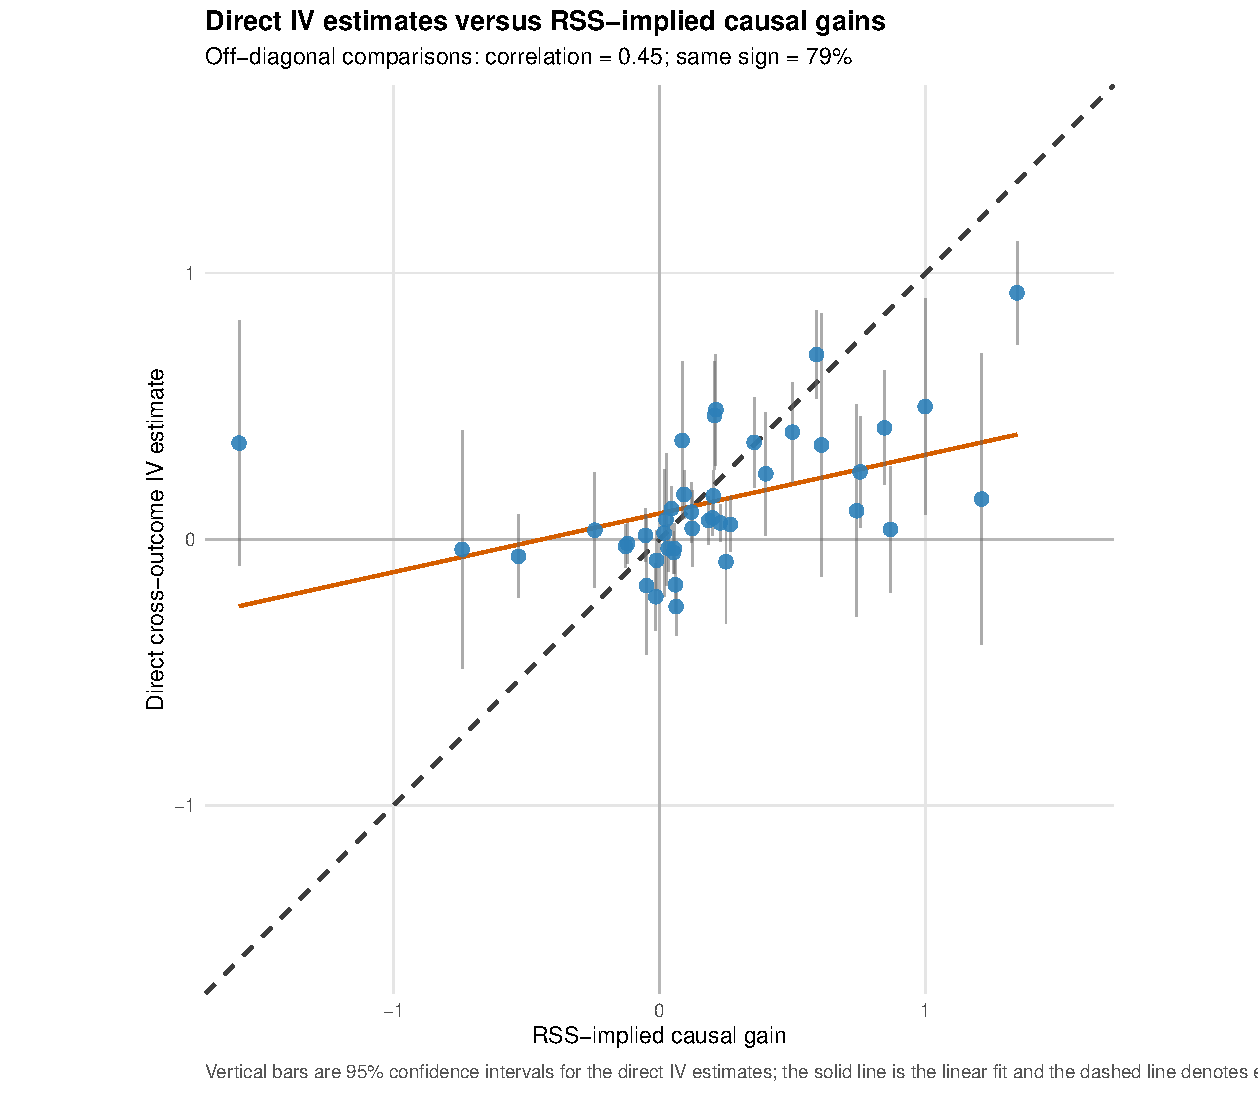
\includegraphics[width=.72\textwidth]{../../output/figures/rss_debiased_varcov/unshrunk_cross_outcome_iv_rss_validation.pdf}
\caption{RSS-implied causal gains and direct cross-outcome IV estimates}
\label{fig:unshrunk-cross-iv-rss-validation}
\begin{minipage}{\textwidth}
\footnotesize \textit{Notes:} Points compare direct cross-outcome IV estimates with RSS-implied causal gains. 
Vertical bars are 95\% confidence intervals for the direct IV estimates; the solid line is the
linear fit and the dashed line denotes exact agreement.
\end{minipage}
\end{figure}


Table~\ref{tab:unshrunk-cross-iv-rss-notable-pairs} illustrates the comparison for ten economically relevant pairs. 
The full set of direct-to-implied ratios is reported in Appendix Table \ref{tab:unshrunk-cross-iv-rss-validation-ratios}.

\begin{table}[!htbp]
\centering
\caption{Selected cross-outcome relationships and direct IV validation}
\label{tab:unshrunk-cross-iv-rss-notable-pairs}
\resizebox{\textwidth}{!}{%
\begin{tabular}{llcccc}
\toprule
Conceptual link & School VA $\rightarrow$ outcome & RSS projection & RSS-implied gain & Direct IV & Direct / implied \\
\midrule
Academic complementarities & Math $\rightarrow$ Verbal & 0.62 & 0.59 & 0.69 & 1.17 \\
 &  & (0.01) &  & (0.08) &  \\
Academic complementarities & Verbal $\rightarrow$ Math & 1.18 & 1.34 & 0.93 & 0.69 \\
 &  & (0.03) &  & (0.10) &  \\
Academic preparation and access & Math $\rightarrow$ Exam taking & 0.10 & 0.05 & 0.12 & 2.54 \\
 &  & (0.01) &  & (0.04) &  \\
Academic preparation and access & Verbal $\rightarrow$ Exam taking & 0.20 & 0.09 & 0.17 & 1.82 \\
 &  & (0.01) &  & (0.05) &  \\
Access complementarities & Exam taking $\rightarrow$ Higher-ed enrollment & 0.41 & 0.27 & 0.06 & 0.21 \\
 &  & (0.01) &  & (0.05) &  \\
Access complementarities & Fin. aid app. $\rightarrow$ Higher-ed enrollment & 0.33 & 0.21 & 0.49 & 2.29 \\
 &  & (0.03) &  & (0.11) &  \\
Postsecondary complementarities & High-premium inst. $\rightarrow$ High-premium field & 0.12 & 0.09 & 0.37 & 4.35 \\
 &  & (0.02) &  & (0.15) &  \\
Postsecondary complementarities & High-premium field $\rightarrow$ High-premium inst. & 0.30 & 0.20 & 0.16 & 0.81 \\
 &  & (0.04) &  & (0.05) &  \\
Access and postsecondary choice & Higher-ed enrollment $\rightarrow$ High-premium inst. & 0.18 & 0.12 & 0.04 & 0.33 \\
 &  & (0.06) &  & (0.07) &  \\
Access and postsecondary choice & Higher-ed enrollment $\rightarrow$ High-premium field & 0.35 & 0.25 & -0.08 & -0.34 \\
 &  & (0.03) &  & (0.12) &  \\
\bottomrule
\end{tabular}}
\par\medskip
\footnotesize
\begin{minipage}{\textwidth}
\textit{Notes:} The table reports ten pairs chosen a priori to represent five economically relevant links. The implied gain multiplies the RSS row-to-column projection by the destination outcome's same-outcome IV pass-through. Parentheses contain bootstrap standard errors for RSS projections and regression standard errors for direct IV estimates. A direct-to-implied ratio of one denotes exact agreement.
\end{minipage}
\end{table}


%For completeness, Table~\ref{tab:unshrunk-cross-iv-rss-validation-ratios} reports the direct-to-implied ratio for every directed pair. Values near one indicate close agreement, values near zero indicate little direct IV effect relative to the RSS prediction, and negative values indicate opposite signs. The ratio matrix is best interpreted together with the levels in Table~\ref{tab:unshrunk-cross-iv-rss-validation}, since ratios can become very large when the RSS-implied gain is close to zero. Diagonal entries equal one mechanically and therefore provide no validation evidence.


%As a complementary check, I compute how much of each outcome's raw correlation with math value added survives after removing the debiased linear projection onto math, using the pooled (non-cross-cohort) value-added estimates from equation~\eqref{eq:observational-va} and the debiased slope $\widehat\beta^{\,m\mid \text{math}}$ from equation~\eqref{eq:varcov-implied-gain}.
%For high-premium-institution value added, the naive correlation with math value added is 0.469 before removing the math component and 0.008 after; for high-premium-field value added, 0.232 before and $-0.024$ after; for log-income value added, 0.425 before and $-0.074$ after; for admission-exam-taking value added, 0.229 before and $-0.026$ after; and for financial-aid-application value added, $-0.281$ before and 0.004 after.
% [UNCLEAR] This exercise reads as close to mechanical: removing the projection on math with (approximately) the population slope should leave near-zero correlation with math by construction. As written it isn't evidence of anything; clarify what it adds or cut it.
%In every case, the residual correlation after removing the debiased math projection is close to zero, an order of magnitude smaller than the correlation it started from.
%This means the debiased implied-gain coefficient captures nearly all of the linear association between math value added and each of the other outcomes: whatever additional signal these outcomes' value-added measures contain is, by construction, orthogonal to math value added rather than a residual piece of it.

Taken together, these results support the paper's motivating claim that school effects on higher-education choices are not simply a noisy reflection of school effects on achievement.
Achievement, postsecondary access, institution choice, and field choice are related but distinct dimensions of school effectiveness. 
Even two outcomes that might appear closely connected---placing students in high-premium institutions and placing them in high-premium fields---are only weakly related across schools.

This matters for how school quality is interpreted. 
A ranking based on achievement value added contains some information about schools' effects on later outcomes, but it is far from a sufficient summary. 
Schools that look similar when ranked by achievement can have very different effects on whether students enter higher education and on the institutions and fields they ultimately choose.
%\subsection{Heterogeneity by Baseline Achievement}

%Figure~\ref{fig:simce4-math-quintile-primary-five-eb} repeats the five primary EB estimates separately by quintiles of baseline grade-4 math achievement.
%This comparison is useful because it keeps the heterogeneity split pre-treatment and available for the full exam-taker analysis sample.
%Table~\ref{tab:simce4-math-quintile-primary-five-eb-contrasts-q3} formally tests each quintile coefficient against the middle quintile, reporting $\widehat{\psi}^{EB}_{Q_q}-\widehat{\psi}^{EB}_{Q_3}$ for $q\in\{1,2,4,5\}$.
%
%The clearest heterogeneity appears in math.
%The bottom-quintile estimate is 0.083, compared with 0.929 in the middle quintile, a difference of $-0.846$ ($p<0.01$).
%The top-quintile estimate is 1.285, or 0.356 above the middle quintile, although this difference is significant only at the 10 percent level ($p=0.093$).
%The math estimates for the second and fourth quintiles are not statistically different from the middle-quintile estimate.
%These results suggest a limit to the constant-effects model of schools, but also efficiency and equity considerations on policies based on value-added reporting.
%Low baseline achievement students might severely underestimate the gains from switching schools, rendering those moves as less efficient or even detrimental if we consider switching costs.
%
%None of the four contrasts with the middle quintile is statistically significant for verbal, high-premium-institution enrollment, high-premium-field enrollment, or log projected program income.
%Thus, the formal tests support meaningful heterogeneity in math, but an almost flat gradient across the higher-education outcomes by baseline achievement.
%
%\begin{figure}[!htbp]
%\centering
%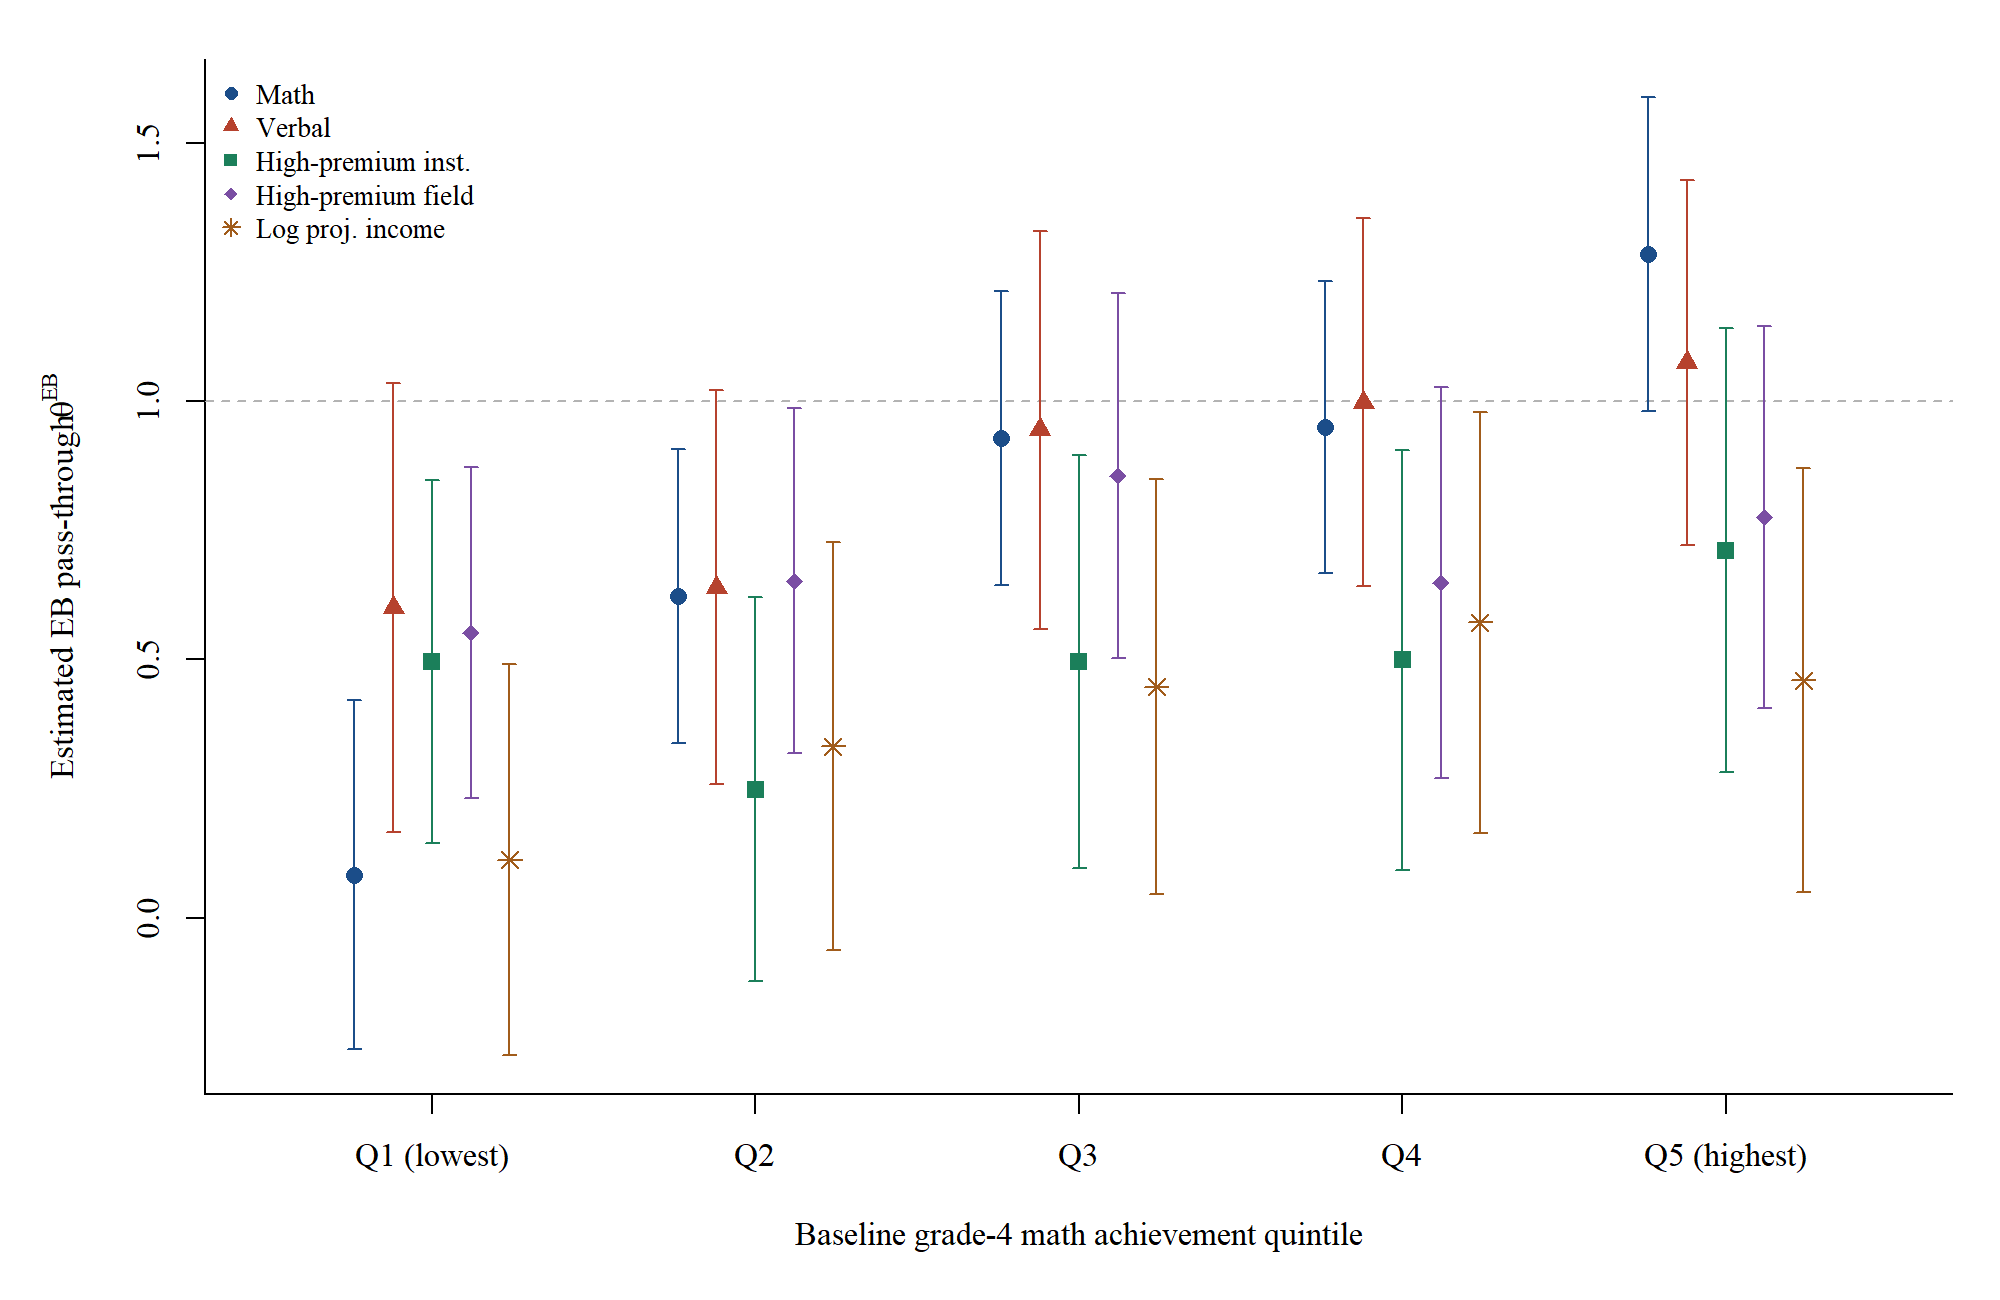
\includegraphics[width=.9\textwidth]{../../output/figures/results_section/simce4_math_quintile_primary_five_eb.png}
%\caption{EB scalar school-value IV estimates by baseline grade-4 math achievement quintile}
%\label{fig:simce4-math-quintile-primary-five-eb}
%\end{figure}
%\begin{table}[!htbp]
\centering
\caption{Differences in EB pass-through relative to the middle quintile}
\label{tab:simce4-math-quintile-primary-five-eb-contrasts-q3}
\small
\resizebox{\textwidth}{!}{%
\begin{tabular}{lccccc}
\toprule
 & \multicolumn{2}{c}{Exams} & \multicolumn{3}{c}{Higher ed. choices} \\
\cmidrule(lr){2-3} \cmidrule(lr){4-6}
Comparison & Math & Verbal & High-premium inst. & High-premium field & Log proj. income \\
\midrule
$Q1-Q3$ & -0.846*** & -0.345 & 0.001 & -0.304 & -0.335 \\
 & (0.225) & (0.296) & (0.272) & (0.243) & (0.282) \\
$Q2-Q3$ & -0.306 & -0.305 & -0.247 & -0.203 & -0.115 \\
 & (0.205) & (0.277) & (0.278) & (0.248) & (0.287) \\
$Q4-Q3$ & 0.022 & 0.053 & 0.003 & -0.207 & 0.125 \\
 & (0.205) & (0.268) & (0.291) & (0.264) & (0.292) \\
$Q5-Q3$ & 0.356* & 0.130 & 0.216 & -0.080 & 0.013 \\
 & (0.212) & (0.267) & (0.300) & (0.261) & (0.293) \\
\bottomrule
\end{tabular}
}
\par\medskip
\footnotesize
\begin{minipage}{\textwidth}
Notes: Each entry reports $\widehat{\theta}^{EB}_{Q_q} - \widehat{\theta}^{EB}_{Q3}$ for the indicated baseline grade-4 math achievement quintile. Heteroskedasticity-robust standard errors are reported in parentheses. Because quintile samples are disjoint, the contrast variance is the sum of the two coefficient variances. $^{*}p<0.10$, $^{**}p<0.05$, $^{***}p<0.01$.
\end{minipage}
\end{table}

%\FloatBarrier
%
%\subsection{Heterogeneity by Gender}
%
%I next ask whether the forecast estimates differ by gender.
%Gender is measured from the grade-8 enrollment records used to construct the linked student panel, so this split is predetermined relative to high-school assignment and does not rely on SAE or admission-test records.
%Figure~\ref{fig:primary-five-eb-by-gender} reports the five EB forecast estimates separately for boys and girls.
%Table~\ref{tab:primary-five-eb-gender-contrasts} reports the corresponding difference, girls relative to boys.
%
%The estimates are positive for both groups across all five outcomes.
%For achievement, however, the point estimates are larger for girls.
%The math pass-through estimate is 0.703 for boys and 1.053 for girls, a difference of 0.349 ($p=0.017$).
%The verbal estimate is 0.685 for boys and 1.066 for girls, a difference of 0.382 ($p=0.029$).
%Thus, lottery-induced movement toward schools with higher achievement value added appears to translate more strongly into measured achievement gains for girls.
%
%For higher-education choices, the gender differences are noticeably smaller.
%The point estimates for high-premium-institution enrollment and high-premium-field enrollment are also larger for girls, but neither difference is statistically significant.
%For log projected program income, the point estimate is slightly larger for boys, and the difference is close to zero.
%Overall, the gender split suggests meaningful heterogeneity in achievement pass-through, but does not provide evidence that the school effects on higher-education choices differ systematically between boys and girls.
%
%\begin{figure}[!htbp]
%\centering
%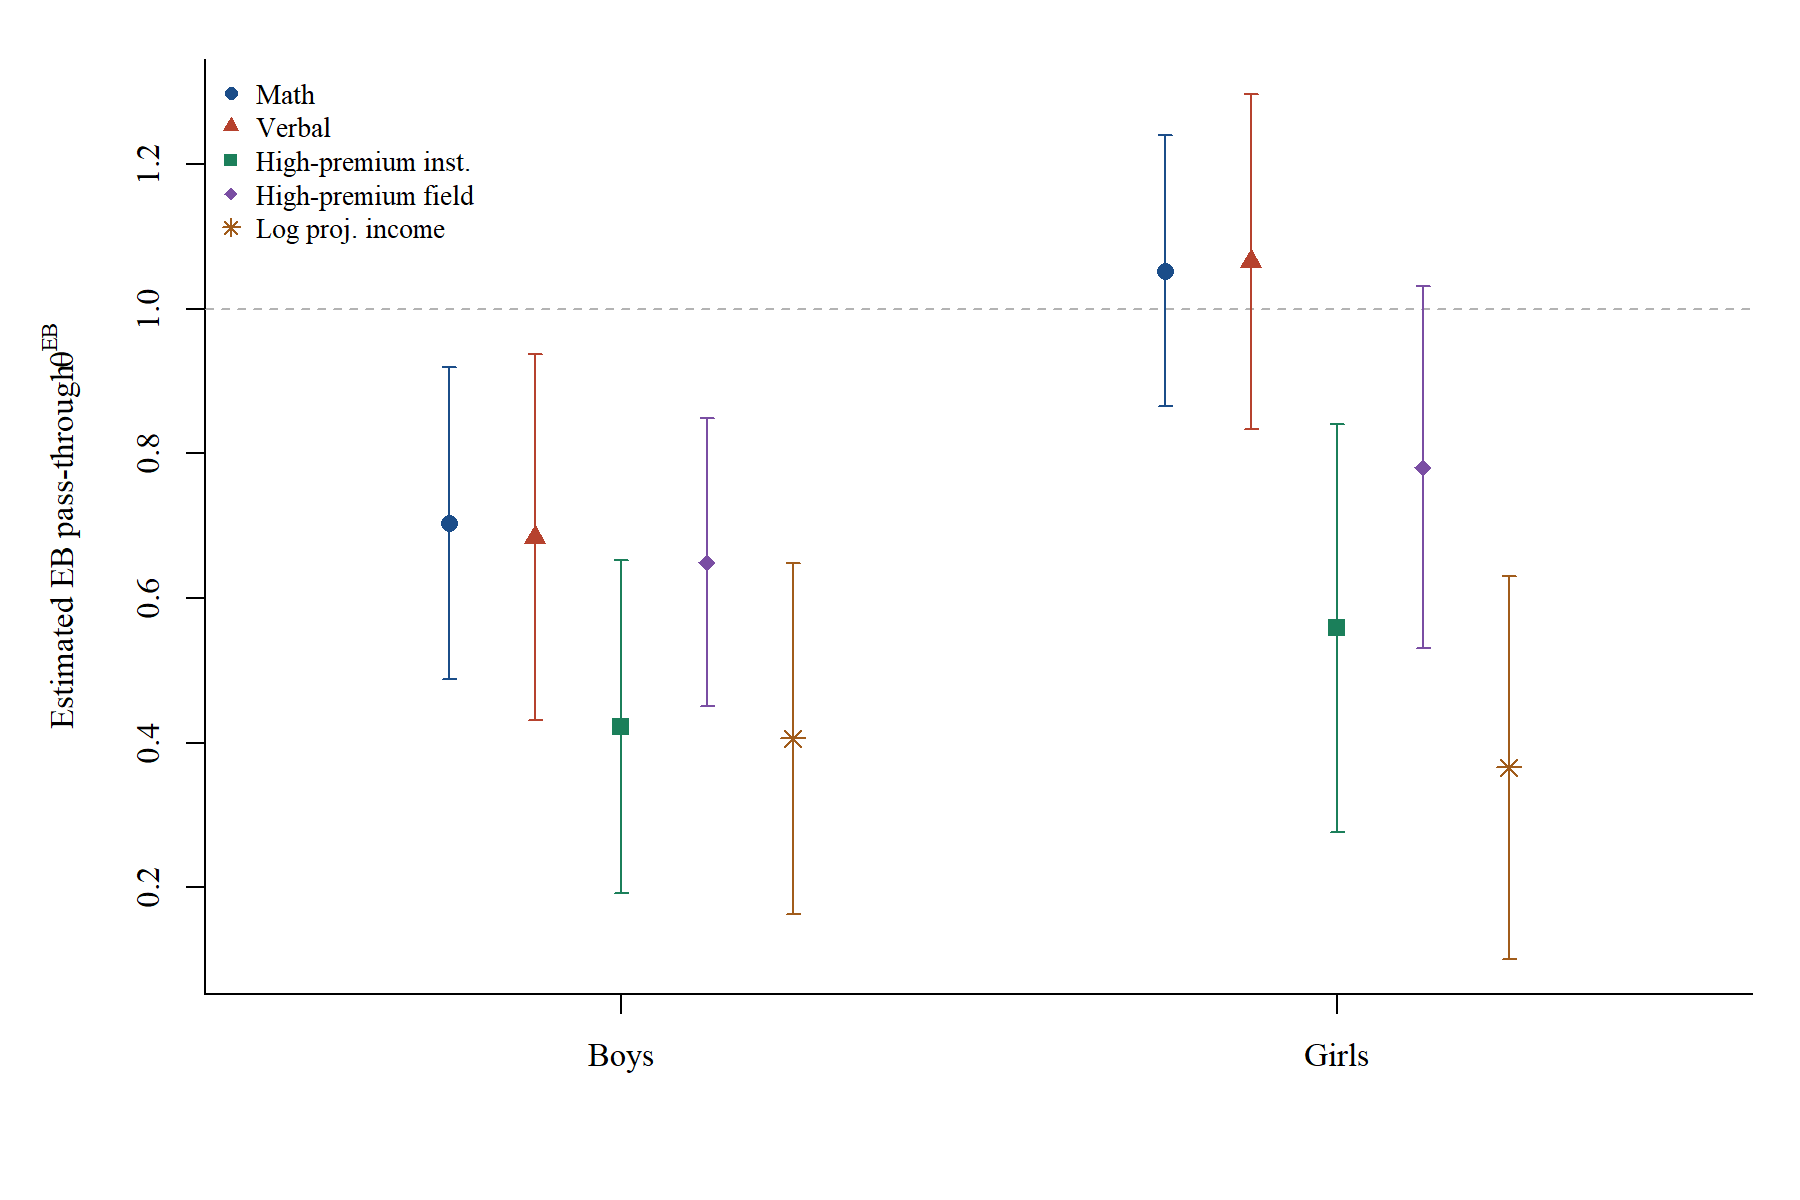
\includegraphics[width=.9\textwidth]{../../output/figures/results_section/primary_five_eb_by_gender.png}
%\caption{EB scalar school-value IV estimates by gender}
%\label{fig:primary-five-eb-by-gender}
%\end{figure}
%\begin{table}[!htbp]
\centering
\caption{Gender differences in EB pass-through}
\label{tab:primary-five-eb-gender-contrasts}
\small
\resizebox{\textwidth}{!}{%
\begin{tabular}{lccccc}
\toprule
 & \multicolumn{2}{c}{Exams} & \multicolumn{3}{c}{Higher ed. choices} \\
\cmidrule(lr){2-3} \cmidrule(lr){4-6}
Comparison & Math & Verbal & High-premium inst. & High-premium field & Log proj. income \\
\midrule
Girls $-$ Boys & 0.349** & 0.382** & 0.137 & 0.131 & -0.040 \\
 & (0.146) & (0.175) & (0.186) & (0.163) & (0.183) \\
\bottomrule
\end{tabular}
}
\par\medskip
\footnotesize
\begin{minipage}{\textwidth}
Notes: Each entry reports the difference in the EB pass-through estimate for girls relative to boys. Heteroskedasticity-robust standard errors are reported in parentheses. Because the two gender samples are disjoint, the contrast variance is the sum of the two coefficient variances. $^{*}p<0.10$, $^{**}p<0.05$, $^{***}p<0.01$.
\end{minipage}
\end{table}

%\FloatBarrier
%
%
%
%\subsection{Ordered Value-Added Horse Race for Projected Income}
%
%The scalar estimates above treat each outcome-specific value-added measure one at a time.
%I next ask whether the labor-market-relevant signal in projected program income is exhausted by math value added.
%This is a stricter question than asking whether schools affect projected income in the scalar specification.
%Schools that raise math achievement may also raise projected income, but high schools may affect later labor-market prospects through other margins: the institutions students attend and the fields they enter.
%The ordered horse race therefore tests which value-added dimensions retain predictive content for projected income as additional dimensions are added.
%
%Figure~\ref{fig:va-correlation-panels}, panel (a), first compares math and verbal value added as an achievement benchmark.
%The two achievement measures are strongly related across schools, with a correlation of 0.659.
%Panel (b) then compares math value added with high-premium-field value added.
%That relationship is positive but much weaker, with a correlation of 0.273.
%This pattern suggests that field-choice value added is related to, but not reducible to, achievement value added.
%The ordered exercise below asks whether these less achievement-like dimensions carry signal for projected income once math value added is given the first place in the ordering.
%
%\begin{figure}[!htbp]
%\centering
%\subbottom[Math and verbal value added\label{fig:math-verbal-va-correlation}]{%
%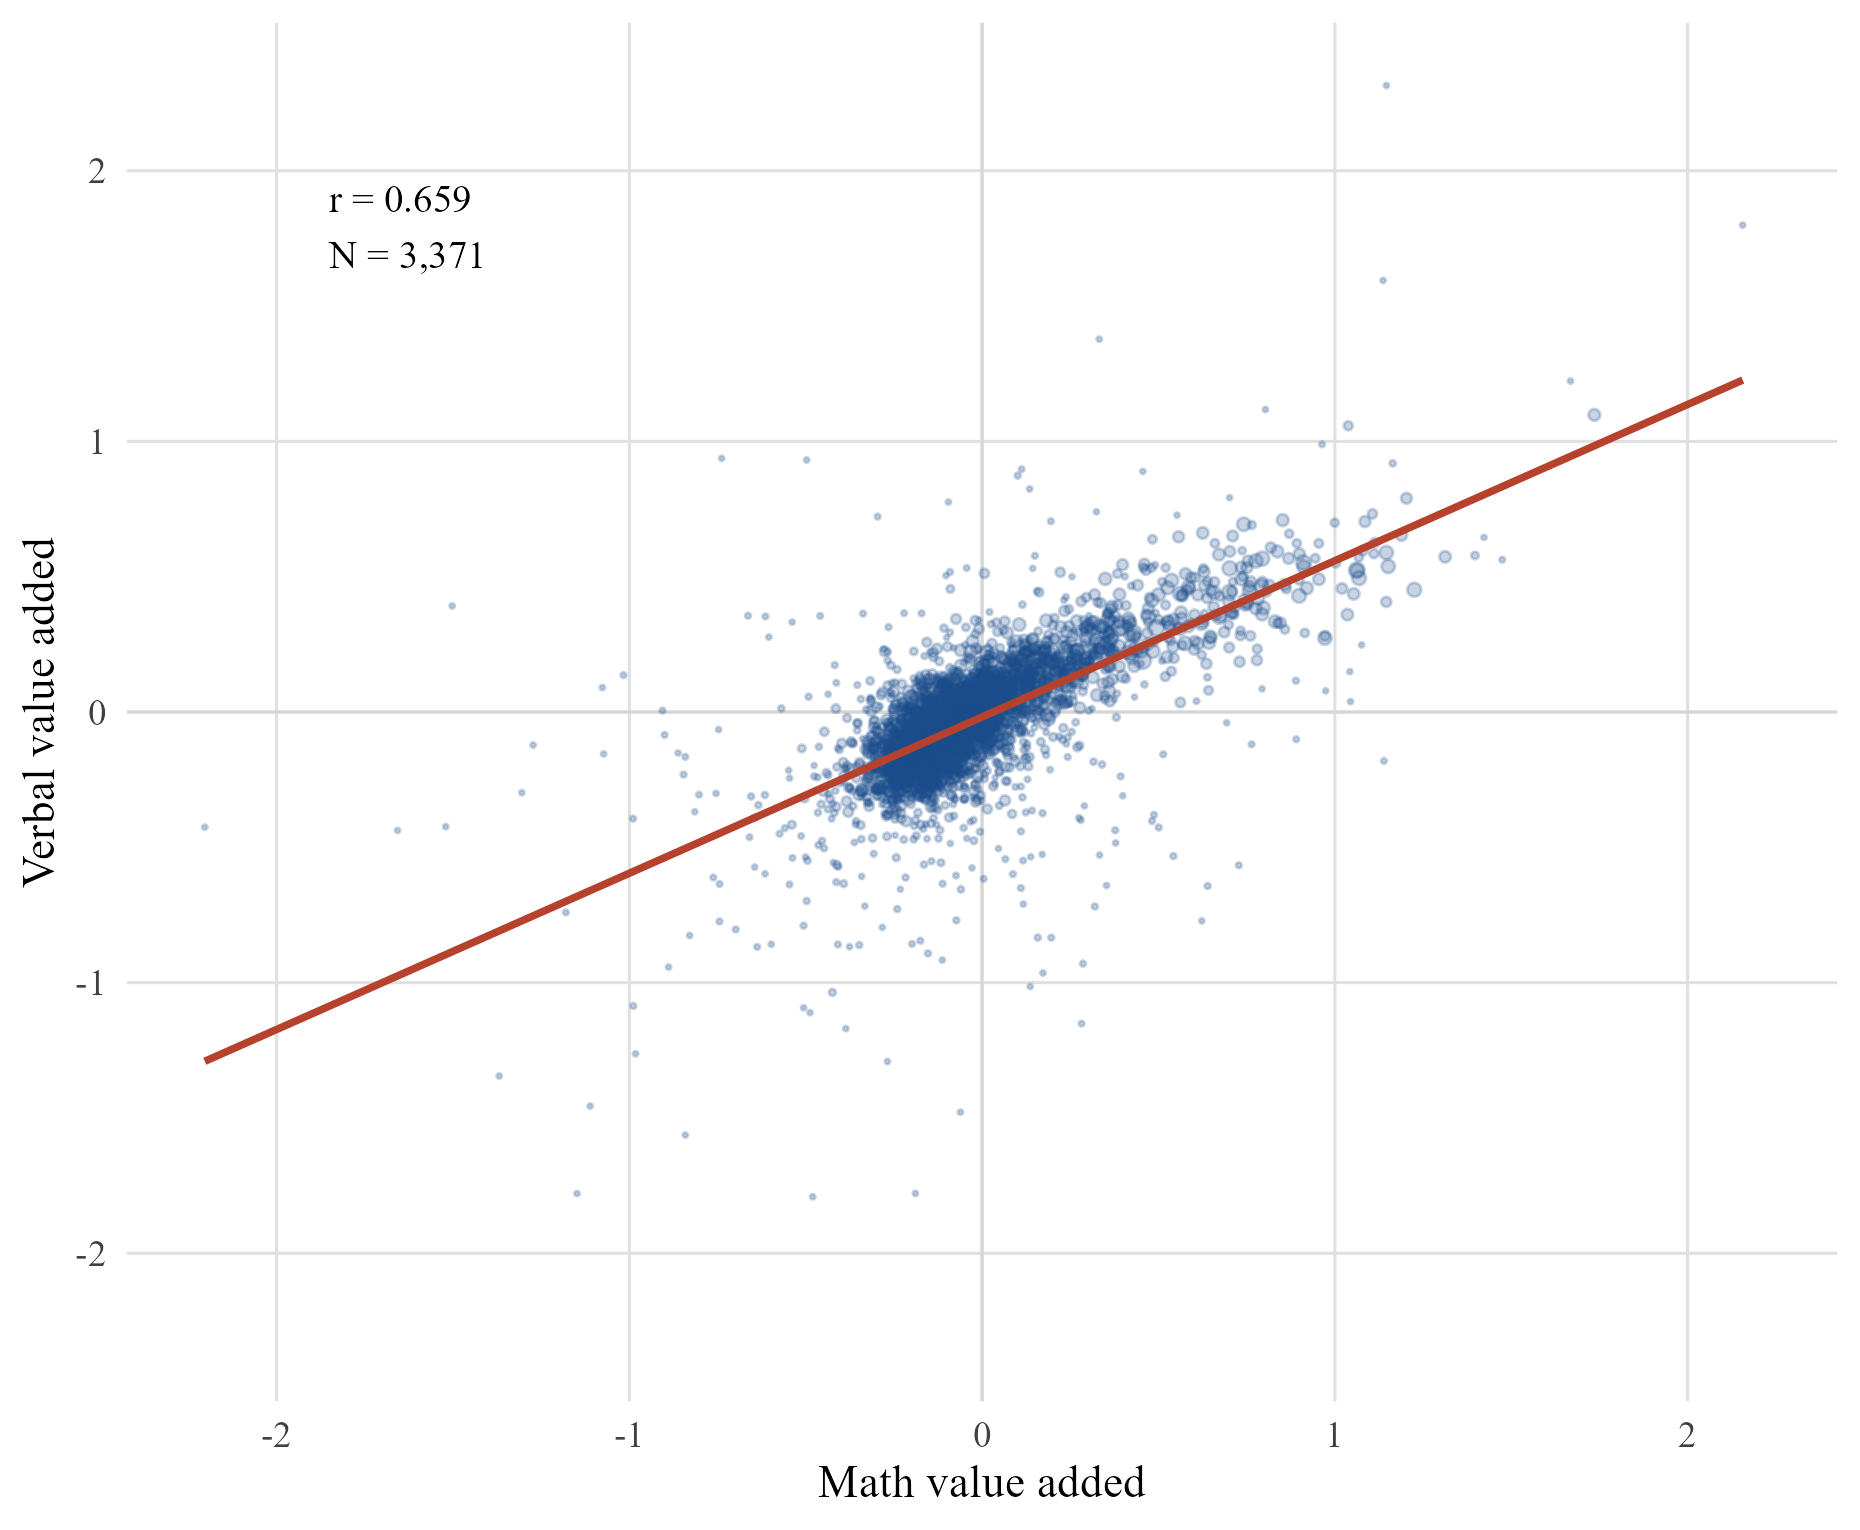
\includegraphics[width=.48\textwidth]{../../output/figures/results_section/math_language_va_correlation.png}%
%}
%\hfill
%\subbottom[Math and high-premium-field value added\label{fig:math-highpay-va-correlation}]{%
%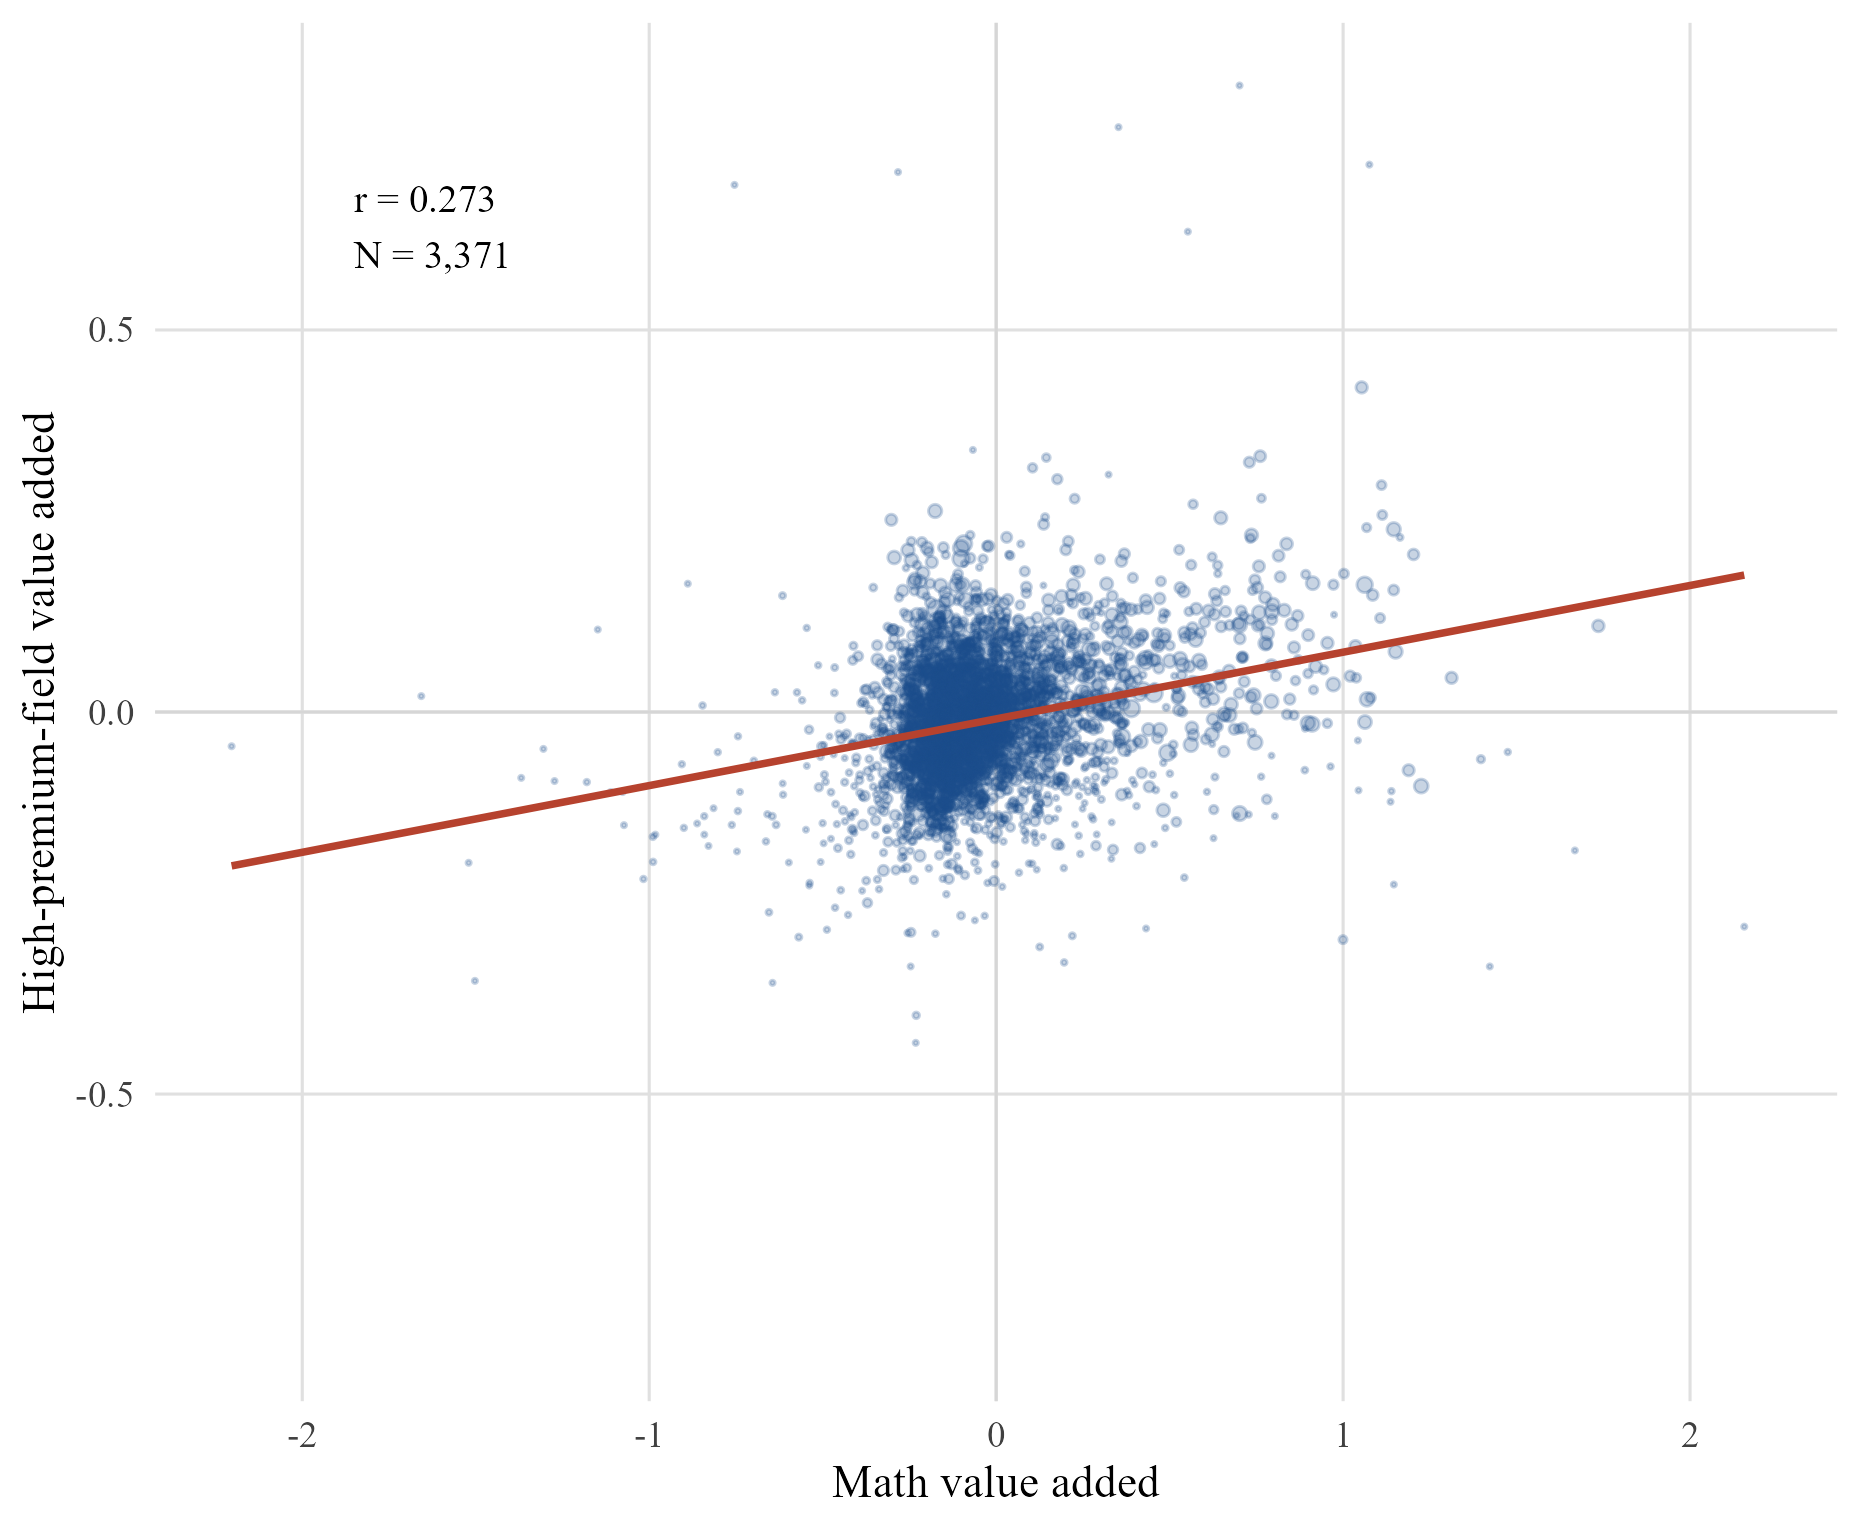
\includegraphics[width=.48\textwidth]{../../output/figures/results_section/math_highpay_va_correlation.png}%
%}
%\caption{Relationships between math, verbal, and high-premium-field observational value added}
%\label{fig:va-correlation-panels}
%\end{figure}
%\FloatBarrier
%
%I estimate a joint IV regression for log projected program income using the ordered EB value-added measures specified in equation~\ref{eq:ordered-va-iv}.
%Each attended school value is instrumented with the corresponding first-round offered-school value, and the regression controls for the assignment-risk expected value of each dimension.
%
%Table~\ref{tab:program-income-orthogonal-math-highinst-highpay} reports the estimates.
%Math value added has a small and statistically insignificant coefficient of $-0.056$.
%High-premium-institution value added net of math is positive, with an estimate of 0.286.
%High-premium-field value added net of math and high-premium-institution value added is positive and precisely estimated, with a coefficient of 0.366.
%These estimates are difficult to reconcile with a view in which math value added fully summarizes the school dimensions relevant for projected income.
%Instead, high schools appear to have labor-market-relevant value-added dimensions that are not captured by achievement value added alone.
%%The strongest evidence comes from the incremental high-premium-field dimension: schools that shift students toward high-premium fields also raise projected income after accounting for math and institution-choice value added.
%%The raw joint horse race gives the same qualitative message, but the ordered version makes the incremental interpretation more transparent.
%
%\begin{table}[!htbp]
\centering
\caption{Ordered IV horse race for log projected income}
\label{tab:program-income-orthogonal-math-highinst-highpay}
\begin{tabular}{lc}
\toprule
 & Log proj. income \\
\midrule
Math VA & -0.056 \\
 & (0.057) \\
High-premium-institution VA net of math & 0.286** \\
 & (0.143) \\
High-premium-field VA net of first two & 0.366*** \\
 & (0.096) \\
\midrule
N & 95,621 \\
\bottomrule
\end{tabular}
\par\medskip
\footnotesize
\begin{minipage}{\textwidth}
Notes: The dependent variable is log projected program income. The table reports an ordered horse-race IV. Math VA enters first; high-premium-institution VA is measured net of math VA; high-premium-field VA is measured net of the first two dimensions. This ordering is used to aid interpretation and does not make the coefficients structural returns to achievement, institutions, or fields. Attended-school values are instrumented with the corresponding first-round offered-school values, and the regression controls for the DA-probability expected value of each dimension, cohort, grade-4 SIMCE math and language, gender, and age. Heteroskedasticity-robust standard errors are reported in parentheses. $^{*}p<0.10$, $^{**}p<0.05$, $^{***}p<0.01$.
\end{minipage}
\end{table}

%
\FloatBarrier

\clearpage 

\section{Conclusion}
\label{sec:conclusion}

High schools shape more than students' academic achievement. 
Using lottery variation from Chile's centralized school assignment system, I show that observational measures of school value added predict causal effects on postsecondary access and higher-education choices as well as on achievement. 
At the same time, these dimensions of school effectiveness are far from interchangeable. 
Schools that improve achievement are not necessarily those that move students toward higher education, and schools that increase enrollment in high-premium institutions are only weakly related to those that increase enrollment in high-premium fields.

This multidimensionality changes how school effects on later choices should be interpreted. 
Decisions about whether to enter higher education, which institution to attend, and which field to study are ultimately made by students. 
But the information, preparation, expectations, and opportunities underlying those decisions may themselves be shaped by the high school attended. 
Postsecondary choices therefore need not simply reveal fixed student preferences; they can also be outcomes of the educational environment that precedes them.

These results also have implications for how school quality is summarized and communicated. 
School rankings and school-choice information are often organized around achievement, implicitly treating test-score performance as a sufficient statistic for school quality. 
The results here suggest that this can be misleading. 
Achievement value added is informative, but it is only imperfectly related to schools' effects on postsecondary access and on the institutions and fields students ultimately choose. 
For families who care about these later outcomes, an achievement-based ranking can therefore give an incomplete picture of the consequences of attending one school rather than another. More generally, there may be no single ranking of high schools that is appropriate for all outcomes students and families care about.

Understanding why schools differ across these dimensions is an important next step. 
The associations with school organization and staff characteristics documented here provide some initial clues, but they do not identify the underlying mechanisms. 
The cohorts studied in this paper are also still early in their postsecondary and labor-market trajectories. 
As additional outcomes become observable, it will be possible to ask whether the school-induced differences in institution and field choice documented here translate into differences in degree completion, earnings, and other longer-run outcomes.
More broadly, understanding what schools produce requires looking not only at what students know when they leave school, but also at the choices they make afterward.

\clearpage
\printbibliography

\clearpage
\section{Appendix}

\begin{table}[!htbp]
\centering
\caption{Ratio of direct cross-outcome IV gains to RSS-implied causal gains}
\label{tab:unshrunk-cross-iv-rss-validation-ratios}
\resizebox{\textwidth}{!}{%
\begin{tabular}{lccccccc}
\toprule
Row school VA & Math & Verbal & Exam taking & Fin. aid app. & Higher-ed enrollment & High-premium inst. & High-premium field \\
\midrule
Math & 1.00 & 1.17 & 2.54 & 0.13 & -1.02 & 0.40 & -2.86 \\
Verbal & 0.69 & 1.00 & 1.82 & 0.21 & -0.62 & 0.27 & -4.02 \\
Exam taking & 0.50 & 0.34 & 1.00 & 0.38 & 0.21 & -0.92 & 15.98 \\
Fin. aid app. & -0.23 & 0.05 & 2.25 & 1.00 & 2.29 & 0.12 & 3.61 \\
Higher-ed enrollment & 0.50 & 0.14 & 0.81 & 1.02 & 1.00 & 0.33 & -0.34 \\
High-premium inst. & 0.13 & 0.58 & 1.34 & -0.14 & 2.97 & 1.00 & 4.35 \\
High-premium field & 0.04 & 0.62 & 7.47 & -0.28 & 0.85 & 0.81 & 1.00 \\
\bottomrule
\end{tabular}}
\par\medskip
\footnotesize
\begin{minipage}{\textwidth}
\textit{Notes:} Entries divide the direct cross-outcome IV estimate by the corresponding RSS-implied causal gain; one denotes exact agreement. Ratios can be unstable when the implied gain is near zero; Table 10 reports the estimates in levels. Diagonal entries equal one mechanically.
\end{minipage}
\end{table}



%\begin{table}[H]
\centering
\caption{Balance by school funding type}
\label{tab:balance_school_sector}
\small
\setlength{\tabcolsep}{4pt}
\begin{tabular}{@{}lccc@{}}
\toprule
 & \shortstack{Broad Panel\\(All HS)} & \shortstack{Public Funding\\HS} & \shortstack{Private\\HS} \\
\midrule
\multicolumn{4}{l}{\textit{Student characteristics}} \\[2pt]
Female & 0.492 & 0.492 & 0.494 \\
Metropolitan Region (Santiago) & 0.387 & 0.366 & 0.588 \\
Age & 13.4 & 13.4 & 13.3 \\
\midrule
\multicolumn{4}{l}{\textit{Baseline SIMCE variables}} \\[2pt]
Math 4th grade (z) & 0.036 & -0.044 & 0.762 \\
Verbal 4th grade (z) & 0.036 & -0.033 & 0.659 \\
Income decile & 5.5 & 5.1 & 9.4 \\
Mother education years & 11.9 & 11.5 & 15.5 \\
\quad\footnotesize{\% matched all SIMCE vars} & \footnotesize{82.4\%} & \footnotesize{81.9\%} & \footnotesize{88.3\%} \\
\midrule
\multicolumn{4}{l}{\textit{Middle school}} \\[2pt]
GPA (z) & 0.032 & 0.029 & 0.070 \\
Attendance (z) & 0.021 & 0.023 & 0.010 \\
\quad\footnotesize{\% matched all middle-school vars} & \footnotesize{99.8\%} & \footnotesize{99.8\%} & \footnotesize{100.0\%} \\
\midrule
\multicolumn{4}{l}{\textit{Outcomes}} \\[2pt]
Std. math exam & 0.000 & -0.155 & 1.085 \\
Std. verbal exam & 0.000 & -0.125 & 0.886 \\
Admission exam taker & 0.776 & 0.761 & 0.932 \\
Higher ed. enrolled & 0.672 & 0.654 & 0.842 \\
Hi-premium institution & 0.128 & 0.089 & 0.508 \\
Hi-premium field & 0.307 & 0.293 & 0.444 \\
\midrule
$N$ & 931,547 & 843,631 &  87,391 \\
Percent of broad panel & 100.0\% & 90.6\% & 9.4\% \\
\bottomrule
\end{tabular}
\par\medskip\footnotesize
\begin{minipage}{\textwidth}
Notes: Broad Panel comprises cohorts 2017--2020 with an observed attended high-school RBD and age 12--16. Public Funding HS includes municipal, local public education service, and subsidized private high schools; Private HS denotes particular pagado high schools. Students with missing school dependency are excluded from both school-type columns. Percentages are relative to the Broad Panel. The SIMCE and middle-school blocks report group means among matched students together with complete-variable match rates. Outcome means use all available observations.
\end{minipage}
\end{table}


%\begin{table}[!htbp]
\centering
\caption{Eventual school by SAE application rank and first-round offer status: VA 2017--2020; SAE 2018--2020}
\label{tab:application-rank-takeup-maximum-data}
\setlength{\tabcolsep}{4pt}
\begin{tabular}{lcccc}
\toprule
\shortstack{Attendance \\
to target school (column), \\ conditional on (row) } & \shortstack{Any of\\top 3} & Choice 1 & Choice 2 & Choice 3 \\
\midrule
Receiving offer & \shortstack{69.5\%\\(N = 140,632)} & \shortstack{39.3\%\\(N = 140,632)} & \shortstack{20.6\%\\(N = 139,954)} & \shortstack{12.7\%\\(N = 116,669)} \\
Not receiving offer  & \shortstack{33.7\%\\(N = 22,001)} & \shortstack{20.1\%\\(N = 22,001)} & \shortstack{8.7\%\\(N = 21,778)} & \shortstack{6.6\%\\(N = 16,961)} \\
\bottomrule
Difference & \textbf{+35.8 pp} & +19.2 pp & +11.9 pp & +6.1 pp \\
\bottomrule
\end{tabular}
\par\medskip
\footnotesize
\begin{minipage}{0.95\textwidth}
Notes: Each cell reports the share whose most-time high school after grade 8 equals the indicated position in the student's SAE application list; the relevant denominator is shown in parentheses. Rank-specific denominators include students who submitted a school at that rank. Received offer means a positive school identifier in the regular first-round SAE assignment record; it does not include later or supplementary assignment rounds. The difference row reports received offer minus did not receive offer.
\end{minipage}
\end{table}





\end{document}
